\pdfoutput=1
\pdfminorversion=6
\documentclass{article}

% if you need to pass options to natbib, use, e.g.:
%\PassOptionsToPackage{numbers, compress}{natbib}
% before loading neurips_2024

\PassOptionsToPackage{numbers, compress}{natbib}
\bibliographystyle{plainnat}

% ready for submission
%\usepackage[preprint]{neurips_2024}


% to compile a preprint version, e.g., for submission to arXiv, add add the
% [preprint] option:
%     \usepackage[preprint]{neurips_2024}


% to compile a camera-ready version, add the [final] option, e.g.:
%     \usepackage[final]{neurips_2024}


% to avoid loading the natbib package, add option nonatbib:
\usepackage[preprint]{neurips_2023}

\usepackage[utf8]{inputenc} % allow utf-8 input
\usepackage[T1]{fontenc}    % use 8-bit T1 fonts
\usepackage{adjustbox}

\usepackage{booktabs}       % professional-quality tables
\usepackage{amsfonts}       % blackboard math symbols
\usepackage{nicefrac}       % compact symbols for 1/2, etc.
\usepackage{microtype} 
\usepackage{graphicx}
\usepackage{hyperref}  

\usepackage{caption}
\usepackage{grffile}
\usepackage{url}            % simple URL typesetting
\usepackage{subcaption}
\usepackage{wrapfig}
\usepackage[dvipsnames]{xcolor}      % colors
\usepackage{multirow}
\usepackage{dsfont}
\usepackage[most]{tcolorbox}
\usepackage{enumitem}
\usepackage{listings}
\hypersetup{
    colorlinks = true,
    citecolor = BlueViolet,
    linkcolor = BrickRed
}
\usepackage{pythonhighlight}

\newcommand\blfootnote[1]{%
  \begingroup
  \renewcommand\thefootnote{}\footnote{#1}%
  \addtocounter{footnote}{-1}%
  \endgroup
}

% \title{Automatic jailbreaking the Image Generative AI}
\title{Automatic Jailbreaking of the\\ Text-to-Image Generative AI Systems}


% The \author macro works with any number of authors. There are two commands
% used to separate the names and addresses of multiple authors: \And and \AND.
%
% Using \And between authors leaves it to LaTeX to determine where to break the
% lines. Using \AND forces a line break at that point. So, if LaTeX puts 3 of 4
% authors names on the first line, and the last on the second line, try using
% \AND instead of \And before the third author name.


\author{%
    Minseon Kim$^1$, Hyomin Lee$^2$, Boqing Gong$^3$, Huishuai Zhang$^4$, Sung Ju Hwang$^{1,5}$ \\
    $^1$KAIST, $^2$Korea University, $^4$Peiking University $^5$DeepAuto.ai \\
    \texttt{\{minseonkim, sjhwang82\}@kaist.ac.kr,} 
    \texttt{lhm1024@korea.ac.kr,} \\
    \texttt{boqinggo@outlook.com, zhanghuishuai@pku.edu.cn}
}


\begin{document}

%\usepackage{natbib}
\maketitle

\begin{abstract}
Segment Anything Model 2 (SAM 2) has emerged as a powerful tool for video object segmentation and tracking anything. Key components of SAM 2 that drive the impressive video object segmentation performance include a large multistage image encoder for frame feature extraction and a memory mechanism that stores memory contexts from past frames to help current frame segmentation. The high computation complexity of multistage image encoder and memory module has limited its applications in real-world tasks, e.g., video object segmentation on mobile devices. To address this limitation, we propose EfficientTAMs, lightweight track anything models that produce high-quality results with low latency and model size. Our idea is based on revisiting the plain, nonhierarchical Vision Transformer (ViT) as an image encoder for video object segmentation, and introducing an efficient memory module, which reduces the complexity for both frame feature extraction and memory computation for current frame segmentation. We take vanilla lightweight ViTs and efficient memory module to build EfficientTAMs, and train the models on SA-1B and SA-V datasets for video object segmentation and track anything tasks. We evaluate on multiple video segmentation benchmarks including semi-supervised VOS and promptable video segmentation, and find that our proposed EfficientTAM with vanilla ViT perform comparably to SAM 2 model (HieraB+SAM 2) with $\sim$2x speedup on A100 and $\sim$2.4x  parameter reduction. On segment anything image tasks, our EfficientTAMs also perform favorably over original SAM with $\sim$20x  speedup on A100 and $\sim$20x  parameter reduction. On mobile devices such as iPhone 15 Pro Max, our EfficientTAMs can run at $\sim$10 FPS for performing video object segmentation with reasonable quality, highlighting the capability of small models for on-device video object segmentation applications. 
\end{abstract}
\section{Introduction}
Reinforcement Learning from Human Feedback (RLHF) is a technique that can be used to align an agent --- such as a Large Language Model (LLM) --- to human preferences and lead to more truthful, more helpful, less harmful and more preferred outputs \cite{ouyang2022training}. Proximal Policy Optimization (PPO) \cite{schulman2017proximal} and Direct Preference Optimization (DPO) \cite{rafailov2023direct} are two such aligment techniques which have been extensively used to improve the quality of LLM outputs, leading to instruction following agents or chat assistants which are quickly approaching human-baselines in a variety of knowledge and reasoning tasks \cite{open-llm-leaderboard, clark2018think, zellers2019hellaswag, hendrycks2021measuring, lin2022truthfulqa, DBLP:journals/corr/abs-1907-10641, DBLP:journals/corr/abs-2110-14168}.

However, recent research has shown that RLHF may actually hurt an LLM's reasoning abilities rather than improving it. One study \cite{bekbayev2023poison} discovered that performing alignment during the Supervised Fine-Tuning (SFT) stage of training may lead to worse performance on reasoning benchmarks, and another \cite{bai2022training} discovered that SFT alone outperforms RLHF for smaller models with the benefits of RLHF only emerging for models with more than 1 Billion parameters. Ouyang et al. \cite{ouyang2022training} also reports an increased tendency for RLHF models to make up information in closed domain tasks (``hallucination'') compared to models trained with SFT alone.

To combat the the risk of RLHF compromising the abilities of an LLM in favor of producing preferable outputs we introduce Direct Preference Heads (DPH), a novel feature based approach that optimises a reward score produced by the LLM rather than optimising the logits produced by language modelling head. DPH can be used in combination with (or without) existing alignment techniques to allow language models to self-evaluate outputs sampled at inference time and select the highest scoring candidate.

We evaluate the performance of DPH using an efficient 551M parameter LM on a variety of commonsense reasoning and Natural Language Understanding (NLU) tasks. All code used to train our models is available on \anon{\href{https://github.com/Avelina9X/direct-preference-heads}{GitHub}} and we release our model weights on \anon{\href{https://huggingface.co/collections/Avelina/direct-preference-heads-preprint-6612d8a6fa3843352943fd43}{Hugging Face}}.
\vspace{-0.1in}
\section{Preliminary}
\vspace{-0.1in}
%The issue of copyright infringement in text-to-image (T2I) models has gained significant attention as these models become more prevalent. Early studies, such as those by Heikkilä [1], highlighted the risks of T2I models replicating copyrighted images from detailed prompts, emphasizing the need for robust prevention mechanisms. O'Leary [2] discussed the ethical and legal challenges of AI-generated content, advocating for clearer guidelines and regulations. Vincent [3] demonstrated that even general prompts could lead T2I models to generate images similar to copyrighted content, suggesting solutions like filtering training data and post-generation checks. Gao et al. [4] developed an adversarial attack framework to test T2I models, revealing vulnerabilities in many commercial services and calling for improved robustness and compliance protocols.
\paragraph{Copyright.}
Copyright is a legal protection provided to the owners of "original works of authorship", such as literature, music, and art~\citep{uscopyright2024uscopyright, uspto2024copyright}. This protection is granted to owners under the laws with the \textit{exclusive right to reproduce, or distribute} their works for a certain period of time~\citep{cornell106, uscopyright2024uscopyright}. Reproduction includes making copies of the work in any form, and distribution involves making the work available to the public through selling or lending copies. While the use of copyrighted data in AI models has been tacitly accepted for educational purposes, the rise of commercial AI systems has brought significant attention to the issue of copyright infringement~\citep{lawsuit1,lawsuit2NYTimes,lawsuit3Getty}. Opinions on the legal aspects of AI vary, but ethically, generative AI should not violate any of these rights to protect the intellectual property of the owners. 
In academia, numerous efforts have been made for copyright protection, e.g., training data protection~\citep{zhong2023copyright, shan2023glaze}, theoretical guarantees~\citep{bousquet2020synthetic, elkin2023can, vyas2023provable}, guided generation~\citep{schramowski2022safe, kumari2023ablating} and mechanism design~\citep{zhou2024plug, golatkar2024cpr, deng2024economic}. Despite the efforts, we reveals that commercial T2I systems still infringe copyrights despite careful alignment and red-teaming mechanisms. %Our result also suggests that future protection approaches should be studied under the context of carefully constructed prompts from strong attackers. 

\vspace{-0.12in}
\paragraph{Memorization in T2I models.}
Memorization has been known to occur in T2I models, sometimes producing near-exact reproductions of images from the training dataset~\citep{somepalli2023understanding}.~\citet{carlini2023extractdm} introduce the membership inference attack to extract the training dataset of diffusion models, and several works~\citep{somepalli2023diffusion, wen2024detecting, wang2024diagnosis} have been proposed to mitigate these memorization issues. Despite memorization is a well-known phenomenon, the quantitative evaluation of copyright violation in commercial T2I systems is under-explored. Thus, we propose an Automatic Prompt Generation Pipeline (APGP) to induce copyright infringement in these commercial T2I systems to evaluate the copyright violation using a single target image.

\vspace{-0.12in}
\paragraph{Prompt attack in T2I models.}
Previous attack approaches demonstrate the vulnerabilities in T2I diffusion models by attacking prompts to either generate different objects~\citep{maus2023black} or create potentially harmful images~\citep{yang2023sneakyprompt, zhai2024discovering}. Previous studies~\citep{zhang2023investigating} have explored high-risk prompts that increase copyright risks by pruning tokens based on attention scores, highlighting potential copyright risks but not causing direct infringement. In contrast, our method targets commercial T2I systems without accessing their weights, effectively "jailbreaking" these systems to demonstrate vulnerabilities related to exact copyright infringement.
\section{Method}
\label{sec:method}

\begin{figure*}[t]
    \centering
    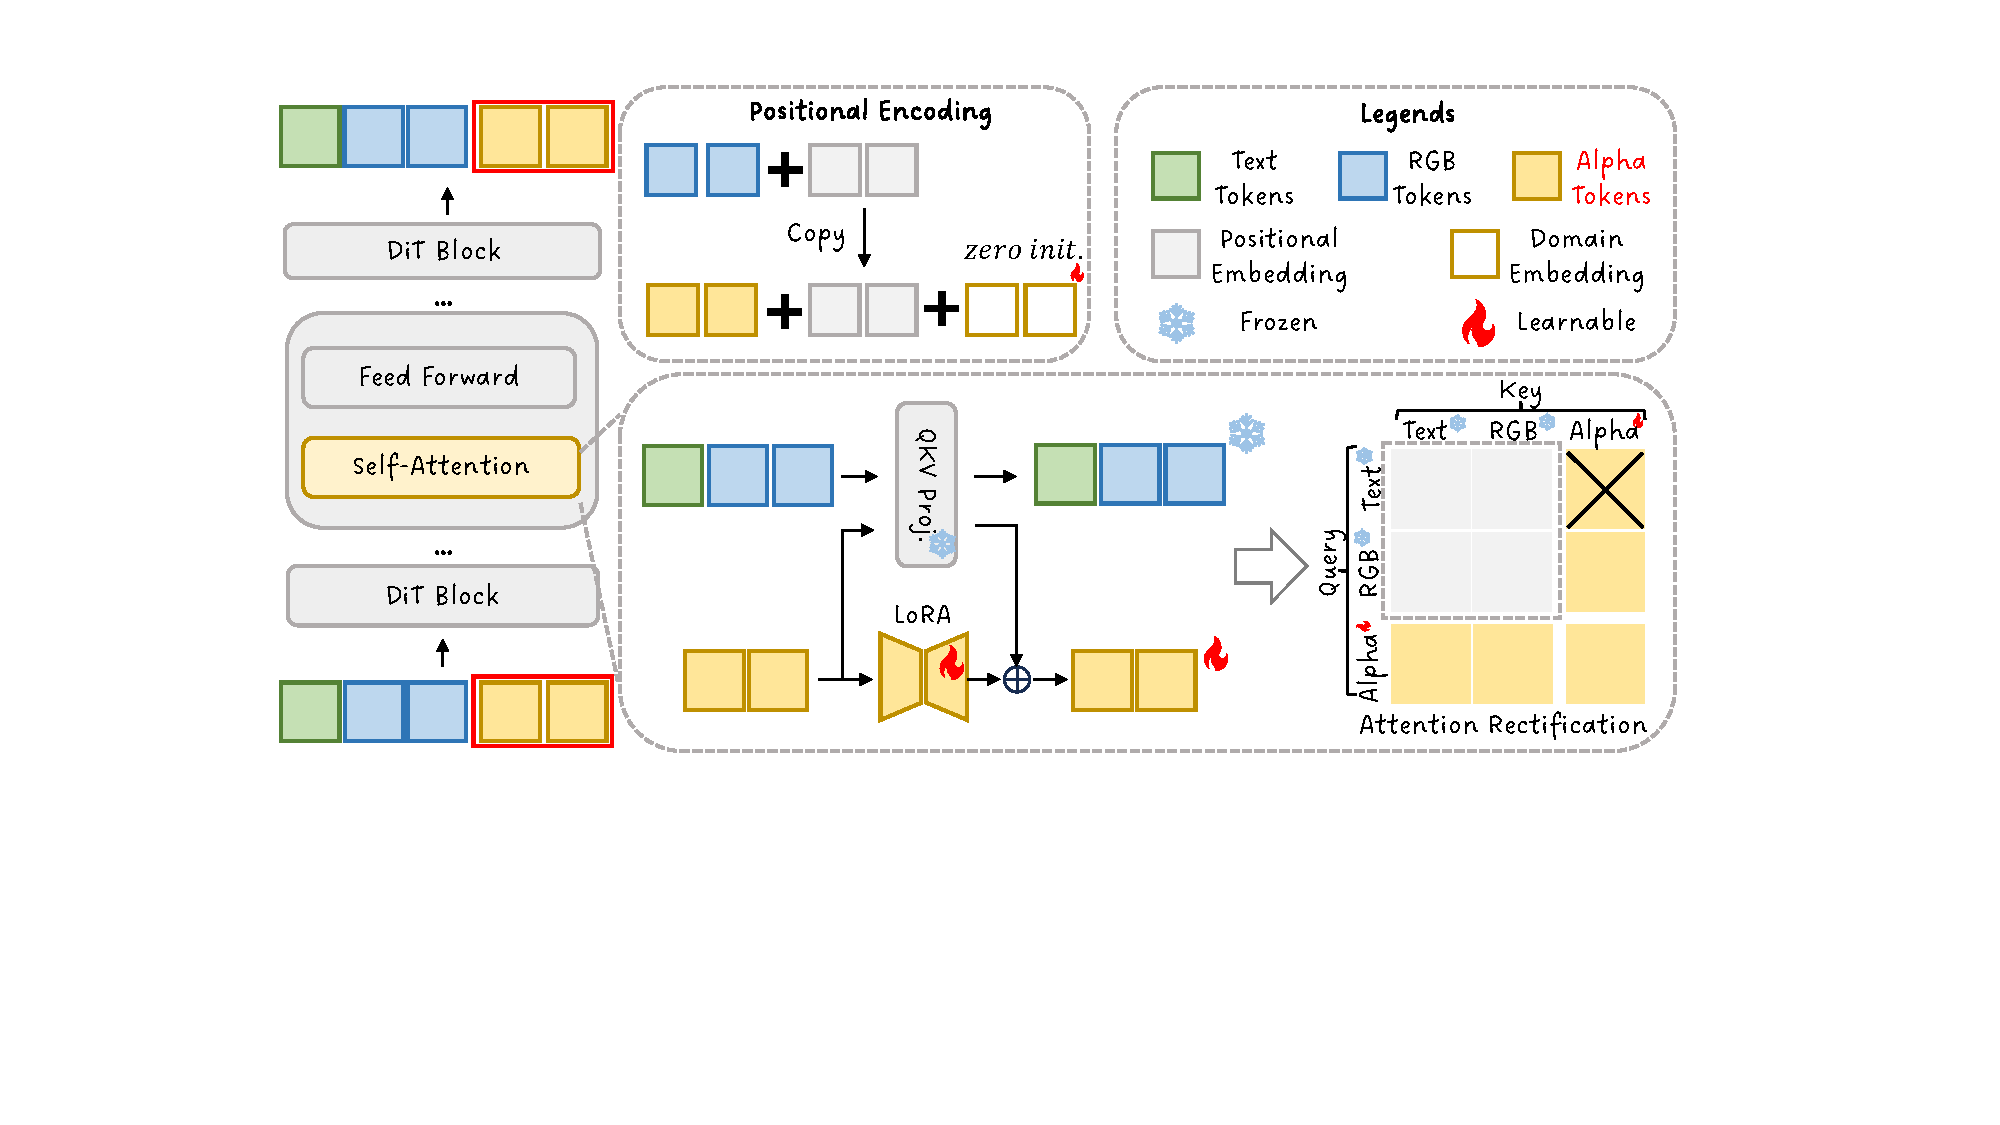
\includegraphics[width=1.0\linewidth]{figs/method-pipeline.pdf}
    \vspace{-0.2in}
    \caption{\textbf{Pipeline of TransPixar.} Our method is organized as follows: (1) \textbf{Left}: we extend the input of DiT to include new alpha tokens; (2) \textbf{Top Center}: we initialize alpha tokens with our positional encoding; (3) \textbf{Bottom Cente}r: we insert a partial LoRA and adjust attention computation during training and inference.}
    \label{fig-pipeline}
    \vspace{-0.1in}
\end{figure*}


% %-------------------------------------------------------------------------
\subsection{Preliminary}
We first introduce the open-sourced state-of-the-art DiT-based video generation models~\cite{yang2024cogvideox,genmo2024mochi}.
The core components of DiT-based video models are attention modules, and there are two primary distinctions between these models and previous approaches.
On one hand, unlike previous models that alternate between 1D temporal attention and 2D spatial attention~\cite{cerspense2023zeroscope, chen2023videocrafter1, chen2024videocrafter2, opensora}, current methods typically employ 3D spatio-temporal attention, allowing them to capture spatio-temporal dependencies more effectively.
On the other hand, instead of using cross-attention for text conditioning, these models concatenate text tokens \( \mathbf{x}_{\text{text}} \) with visual tokens \( \mathbf{x}_{\text{video}} \) into a single long sequence. 
The shape of video tokens and text tokens are \(B\times L\times D\) and \(B\times L_{\text{text}}\times D\), wher \(B\) equals to batch size, \(L_{\text{text}}\) equals to the length of text tokens, \(L\) equals to the length of video tokens and \(D\) equals to the latent dimension of transformer.
Full self-attention is then applied across the combined sequence:
\begin{equation}
\begin{aligned}
    &\text{Attention}(\mathbf{Q}, \mathbf{K}, \mathbf{V}) = \text{softmax}\left(\frac{\mathbf{Q}\mathbf{K}^T}{\sqrt{d_k}}\right)\mathbf{V}, \quad \text{where} \\
&\mathbf{Z : Z \in \{Q, K, V\}} \\&= [\mathbf{W}_{z : z \in \{q, k, v\}}(\mathbf{x}_{\text{text}}); \mathbf{f}_{z : z \in \{q, k, v\}}(\mathbf{x}_{\text{video}})]
\end{aligned}
\label{SA}
\end{equation}


Here \( \mathbf{W}_{t} \) (for \( t \in \{q, k, v\} \)) represents the projection matrixs in the transformer model, and \( \mathbf{f}_{t} \) (for \( t \in \{q, k, v\} \)) represents a combined operation that incorporates both the projection and positional encoding for visual tokens. 
There are two commonly used types of positional encoding. One is absolute positional encoding formulated as follows:
\begin{equation}
\begin{aligned}
\mathbf{f}_{z : z \in \{q, k, v\}}(\mathbf{x}_{\text{video}}) := \mathbf{W}_{z : z \in \{q, k, v\}}(\mathbf{x}_{\text{video}}^m + \mathbf{p}^m),
\end{aligned}
\label{PE}
\end{equation}
where \( \mathbf{p} \) is the positional embedding (e.g., a sinusoidal function) and \( m \) denotes the position of each RGB video token.
Another approach is the Rotary Position Embedding (RoPE)~\cite{su2024roformer}, often used by~\cite{yang2024cogvideox, genmo2024mochi}. 
This is expressed as
\begin{equation}
\begin{aligned}
\mathbf{f}_{z : z \in \{q, k\}}(\mathbf{x}_{\text{video}}) := \mathbf{W}_{z : z \in \{q, k\}}(\mathbf{x}_{\text{video}}^m) \circ e^{im\theta},
\end{aligned}
\label{RoPE}
\end{equation}
where \( m \) is the positional index, \( i \) is the imaginary unit for rotation, and \( \theta \) is the rotation angle.




% %-------------------------------------------------------------------------
\subsection{Our Approach} 
To jointly generate RGB and alpha videos, we adapt a pretrained RGB video generation model through several modifications. The whole pipeline is visualized in Fig.~\ref{fig-pipeline}.

Firstly, we double the sequence length of noisy input tokens to enable the model to generate videos of double length, from \( \mathbf{x}^{1:L}_{\text{video}} \) to \( \mathbf{x}^{1:2*L}_{\text{video}} \). 
Here, \( \mathbf{x}^{1:L}_{\text{video}} \) will be decoded into the RGB video, while \( \mathbf{x}^{L+1:2*L}_{\text{video}} \) will be decoded into the corresponding alpha video.
The Query(Q), Key(K), Value(V) representations are formulated as:
\begin{equation}
\begin{aligned}
&\mathbf{Z : Z \in \{Q, K, V\}} \\&= [\mathbf{W}_{z : z \in \{q, k, v\}}(\mathbf{x}_{\text{text}}); \mathbf{f}_{z : z \in \{q, k, v\}}(\mathbf{x}^{1:2*L}_{\text{video}})]
\end{aligned}
\end{equation}

In addition to sequence doubling, we explored increasing batch size or latent dimensions and splitting output into two domains; however, these approaches showed limited effectiveness under constrained datasets, which we discuss later.

Secondly, we modify the positional encoding function \( \mathbf{f}_{t : t \in \{q, k, v\}}(\cdot) \), as shown in Fig.~\ref{fig-pe}.
Instead of continuously numbering indices, we allow RGB and alpha tokens to share the same positional encoding. 
Taking absolute positional encoding as an example:
\begin{equation}
\begin{aligned}
&\mathbf{f}^*_{z : z \in \{q, k, v\}}(\mathbf{x}_{\text{video}}) \\:=
&\begin{cases}
\mathbf{W}_{z : z \in \{q, k, v\}}(\mathbf{x}_{\text{video}}^m + \mathbf{p}^m), & \text{if } m \leq L, \\
\mathbf{W}^*_{z : z \in \{q, k, v\}}(\mathbf{x}_{\text{video}}^m + \mathbf{p}^{m-L} + d), & \text{if } m > L.
\end{cases}
\label{eq:our_pe}
\end{aligned}
\end{equation}

Here we introduce a domain embedding \( d \), initialized to zero. We make it learnable to help the model adaptively differentiate between RGB (\(m\leq L\)) and alpha tokens (\(m>L \)). 
%
The motivation behind this design is we observe that with same postional encoding, even initializing with different noises, the tokens from two domains tend to generate same results. 
It minimizes spatial-temporal alignment challenges at the very beginning of training and thus accelerates convergence.

Next we propose a fine-tuning scheme using LoRA~\cite{hu2021lora}, in which the LoRA layer is applied only to alpha domain tokens:
\begin{equation}
\begin{aligned}
&\mathbf{W}^*_{z : z \in \{q, k, v\}}(\mathbf{x}_{\text{video}}^m + \mathbf{p}^{m-L} + d)\\=
&\ \mathbf{W}_{z : z \in \{q, k, v\}}(\mathbf{x}_{\text{video}}^m + \mathbf{p}^{m-L} + d)
\\
+\ &\gamma\cdot \text{LoRA}(\mathbf{x}_{\text{video}}^m + \mathbf{p}^{m-L} + d), \quad \text{if } m > L,
\label{eq:our_lora}
\end{aligned}
\end{equation}
where \( \gamma \) controls the residual strength. 
Additionally, we design an attention mask to block unwanted attention computation. 
Given a text-video token sequence length \( L_\text{text} + 2L \), where \( L_\text{text} \) represents text token length, the mask is defined as:
\begin{equation}
\mathbf{M}^*_{mn} = 
\begin{cases} 
-\infty, & \text{if } m \leq L_\text{text} \ \text{and} \ \, n > L_\text{text} + L, \\
0, & \text{otherwise}.
\end{cases}
\label{eq:attn_mask}
\end{equation}

Combining these modifications, inference with our method is expressed as:
\begin{equation}
\begin{aligned}
    &\text{Attention}(\mathbf{Q}, \mathbf{K}, \mathbf{V}) = \text{softmax}\left(\frac{\mathbf{Q}\mathbf{K}^T}{\sqrt{d_k}}+\mathbf{M}^*\right)\mathbf{V}, \quad \text{where} \\
&\mathbf{Z : Z \in \{Q, K, V\}} \\&= [\mathbf{W}_{z : z \in \{q, k, v\}}(\mathbf{x}_{\text{text}}); \mathbf{f}^*_{z : z \in \{q, k, v\}}(\mathbf{x}_{\text{video}})]
\end{aligned}
\label{eq:our_method}
\end{equation}

Training is carried out using flow matching~\cite{liu2022flow} or a traditional diffusion process~\cite{ho2020denoising}.


\begin{figure}[t]
    \centering
    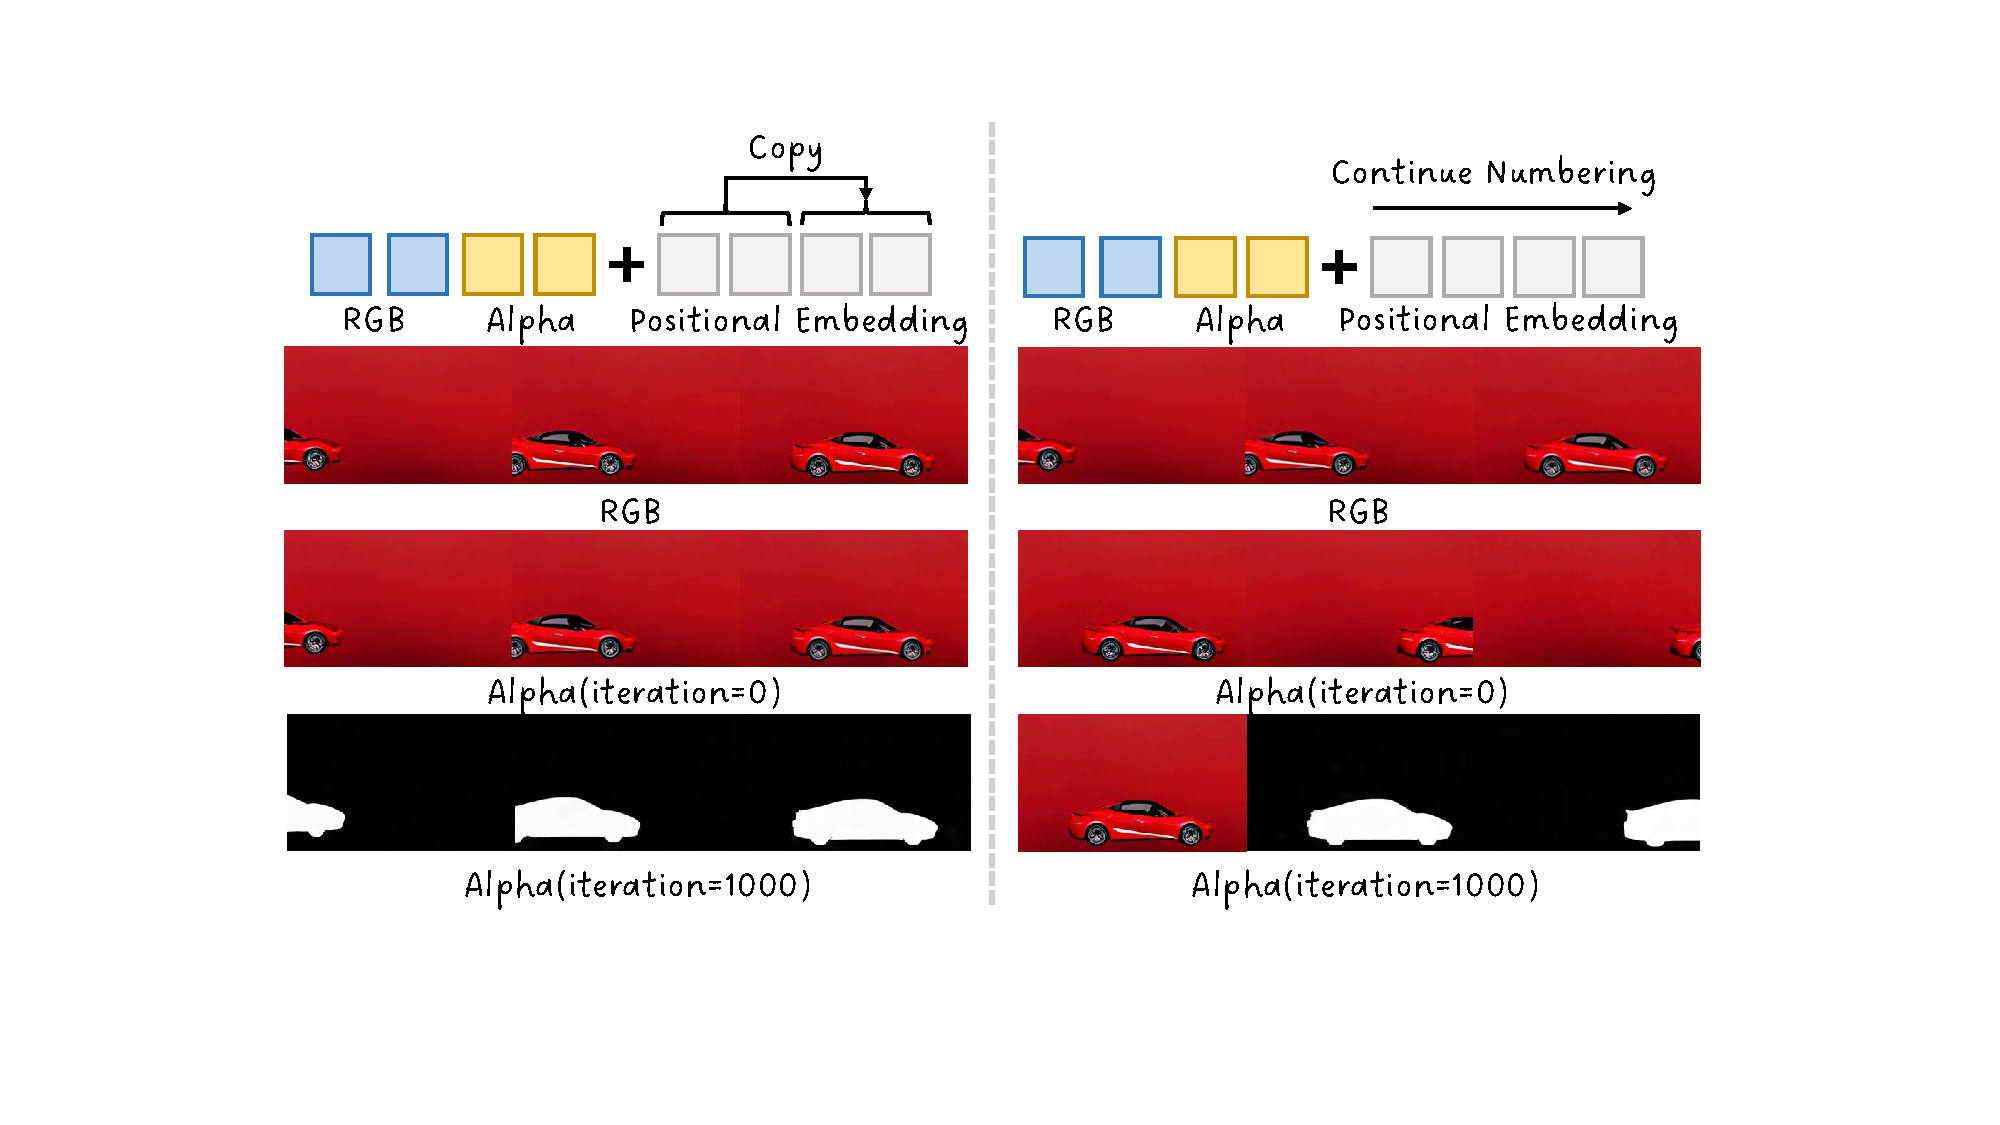
\includegraphics[width=1.0\linewidth]{figs/method-pe_init.pdf}
    \vspace{-0.2in}
    \caption{\textbf{Positional Encoding Design for RGBA Generation.} Assigning alpha tokens the same positional encoding as RGB yields similar results, resulting in faster convergence after 1000 iterations compared to standard encoding strategies.}
    \label{fig-pe}
    \vspace{-0.1in}
\end{figure}

% %-------------------------------------------------------------------------
\subsection{Analysis}
% % given our goal is 最大程度地继承 pretrain video model的能力,让它能生成的东西超越已有的RGBA训练集,
% 在目前我们使用的3d full attention DiT的video generation model的框架下,最重要的计算是attention mechanism,因此我们进一步对该过程进行分析:
% The attention matrix, \(\mathbf{Q}\mathbf{K}^T\), now has dimensions \((L_\text{text} + 2*L) \times (L_\text{text} + 2*L)\), which we simplify by organizing it into a 3x3 grouped attention matrix—\textbf{Text-attend-to-RGB}, \textbf{RGB-attend-to-Text}, and so forth, as illustrated in Fig.~\ref{fig-pipeline}. Then we procceed to analyze them:

% \noindent{\textbf{Text-Attend-to-RGB} and \textbf{RGB-Attend-to-Text}}.
% Given this matrix, we are supposed to preserve as much of the computation in the upper-left 2x2 section as possible so that we can preserve the RGB generation potential. 

% These represent the upper-left 2x2 section in \(\mathbf{Q}\mathbf{K}^T\) and 是RGB original generation model有且仅有的计算过程,如果我们能保证这部分计算不受影响,we can replicate the original RGB generation performance. 
% Therefore, we limited the scope of LoRA's influence, as defined in Equation~\eqref{eq:our_lora}, we retain the original QKV values for both text and RGB tokens, maintaining the pretrained model’s behavior in these domains.

% Besides the partial lora, the introduction of alpha tokens make the text and RGB tokens need to act as key and interact with alpha tokens as query, which will also 改变这个2x2 attention matrix的计算结果。
% Therefore, we proceed to analyze two additional attention computations that affect RGB generation shown in Fig.~\ref{fig-attn}:


% \noindent{\textbf{Text-Attend-to-Alpha}}: We find this attention is detrimental to the generation quality. 
% Since the model is originally trained with text and RGB data, introducing attention from text to alpha causes interference due to the domain gap between alpha and RGB. 
% Specifically, alpha modality provide only contour information and lack the rich texture, color, and semantic details associated with text prompt, thereby degrading generation quality. 
% To mitigate this, we design the attention mask (Equation~\eqref{eq:attn_mask}) that blocks this computation.

% \noindent{\textbf{RGB-Attend-to-Alpha}}: In contrast, we identify \textbf{RGB-to-Alpha} as essential for successful joint generation. 
% This attention allows the model to refine RGB tokens by considering alpha information, facilitating alignment between generated RGB and alpha channels. 
% This refinement process is a critical component missing in prior generation-then-prediction pipelines, which lack a feedback mechanism for RGB refinement based on alpha guidance.
Given our goal of maximizing the inherited capabilities of the pretrained video model, enabling it to generate beyond the existing RGBA training set, we analyze the most critical component within our current 3D full attention DiT video generation model: the attention mechanism.
%
The attention matrix, \(\mathbf{Q}\mathbf{K}^T\), has dimensions \((L_\text{text} + 2*L) \times (L_\text{text} + 2*L)\), which we simplify by organizing it into a 3x3 grouped attention matrix—including \textbf{Text-attend-to-RGB}, \textbf{RGB-attend-to-Text}, and so forth, as illustrated in Fig.~\ref{fig-pipeline}. %We then analyze these components:

\vspace{0.5em}
\noindent\textbf{Text-Attend-to-RGB and RGB-Attend-to-Text}. These represent the upper-left 2x2 section of  and are computations that exist solely in the original RGB generation model. If we ensure that this part of the computation remains unaffected, we can replicate the original RGB generation performance. Therefore, we limit the scope of LoRA's influence, as defined in Eq.~\eqref{eq:attn_mask}, by retaining the original QKV values for both text and RGB tokens, thus preserving the pretrained model’s behavior in these domains.

Besides the partial LoRA, the added alpha tokens requires the text and RGB tokens to also act as queries and interact with the alpha tokens as keys, which alters the computation in this 2x2 attention matrix. 
Therefore, we further analyze two additional attention computations that impact RGB generation, as shown in Fig.~\ref{fig-attn}.

\vspace{0.5em}
\noindent\textbf{Text-Attend-to-Alpha.} We find that this attention is detrimental to the generation quality. Since the model was originally trained with text and RGB data, introducing attention from text to alpha causes interference due to the domain gap between alpha and RGB. Specifically, the alpha modality provides only contour information and lacks the rich texture, color, and semantic details associated with the text prompt, thereby degrading generation quality. To mitigate this, we design the attention mask (Eq.~\eqref{eq:attn_mask}) that blocks this computation.

\vspace{0.5em}
\noindent\textbf{RGB-Attend-to-Alpha.} In contrast, we identify \textbf{RGB-to-Alpha} as essential for successful joint generation. This attention allows the model to refine RGB tokens by considering alpha information, facilitating alignment between generated RGB and alpha channels. This refinement process is a critical component missing in previous generation-then-prediction pipelines, which lacked a feedback mechanism for RGB refinement based on alpha guidance.


\begin{figure}[t]
    \centering
    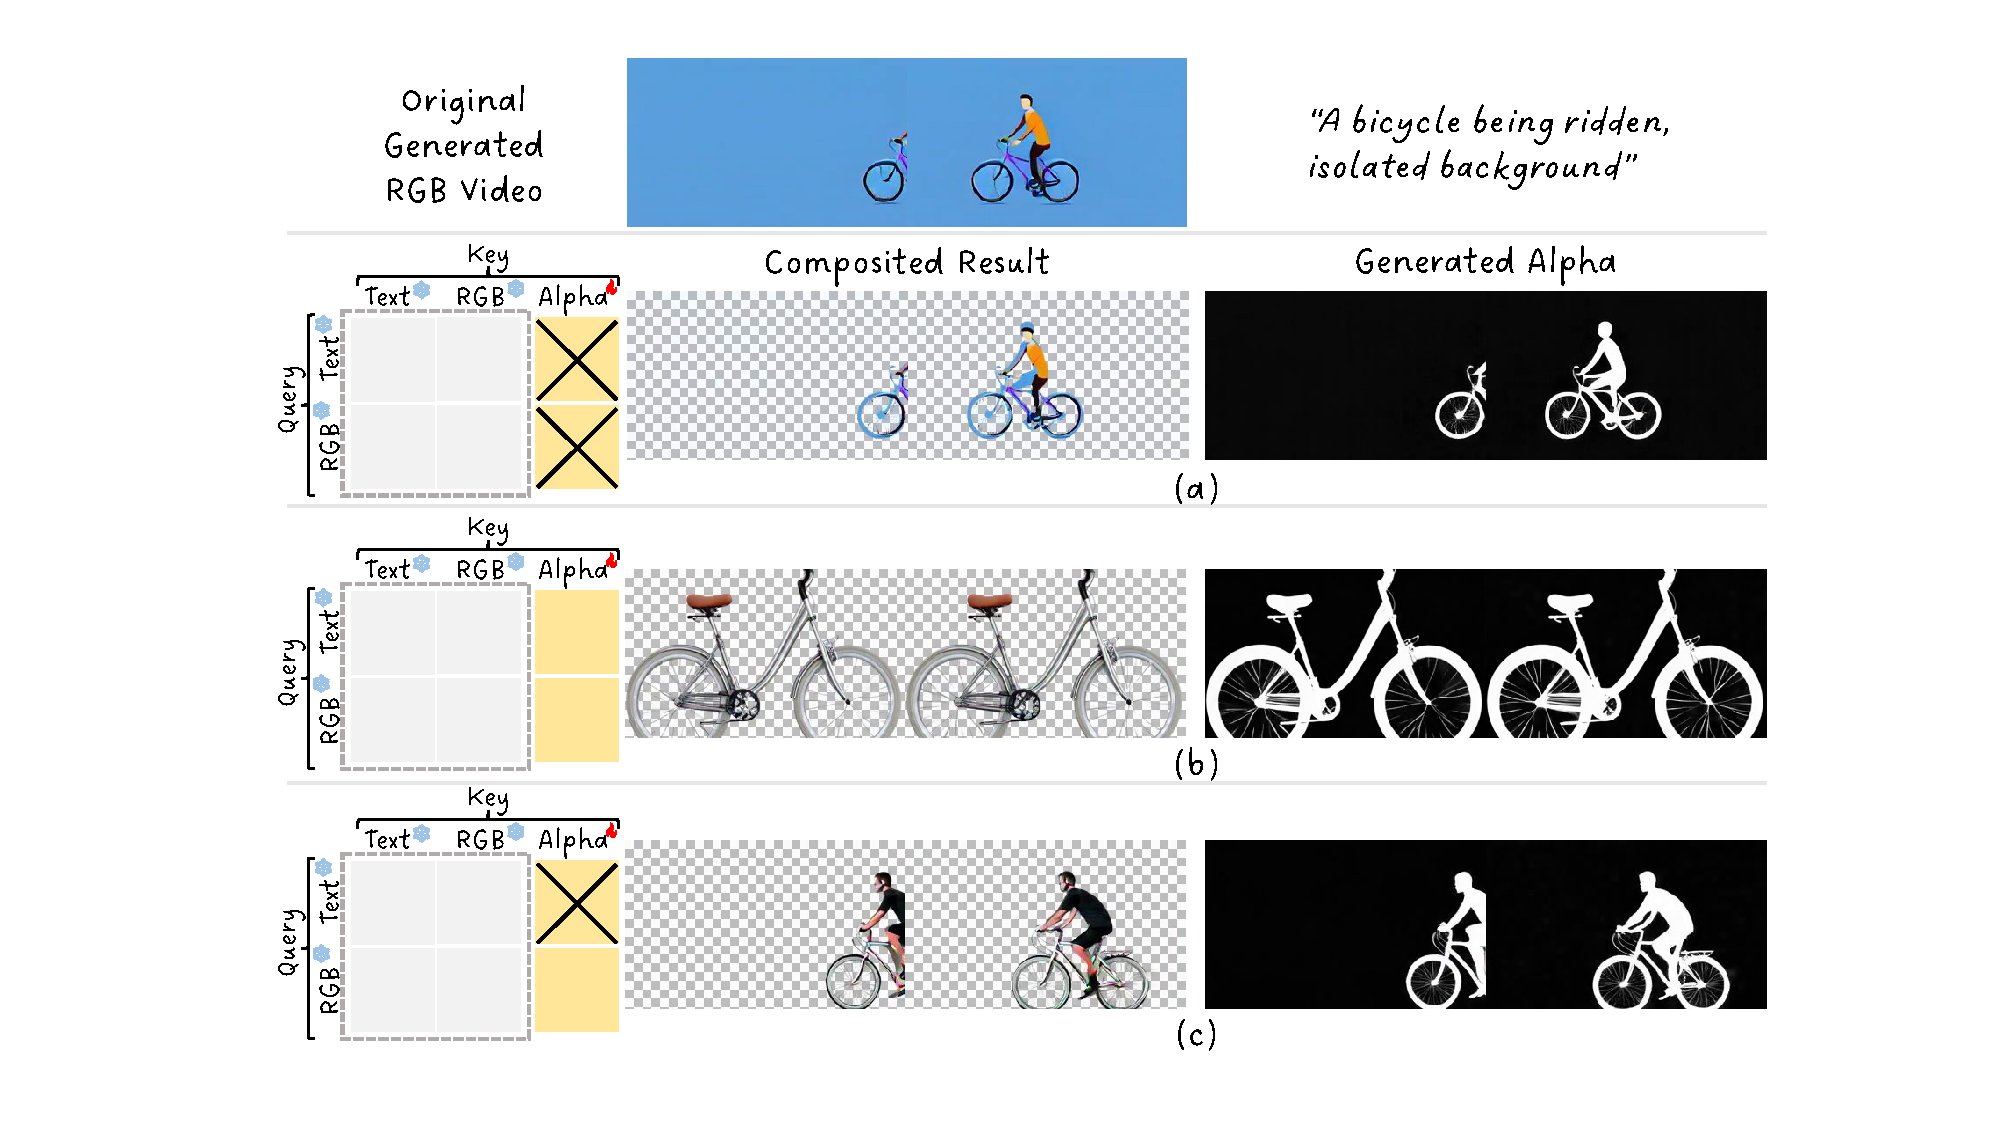
\includegraphics[width=1.0\linewidth]{figs/method-attn.pdf}
    \vspace{-0.2in}
    \caption{\textbf{Attention Rectification.} (a) Eliminating all attention from alpha as a key preserves 100\% RGB generation but leads to poor alignment. (b) Retaining all attention significantly degrades quality, causing a lack of motion in bicycles. (c) Our method achieves an effective balance.
    }
    \label{fig-attn}
    \vspace{-0.1in}
\end{figure}




\vspace{-0.13in}
\section{Experimental results}
\vspace{-0.1in}
In this section, we extensively evaluate the efficacy of our Automated Prompt Generation Pipeline (APGP) on current commercial text-to-image (T2I) systems on the simple prompt in Violation dataset for T2I models (VioT)(Section~\ref{result:simple_prompt}). Furthermore, we extensively evaluate the ChatGPT, specifically GPT-4, on our APGP-generated prompt (Section~\ref{result:our_prompt}). Finally, we further examine whether APGP still exhibits similar performance against simple defense mechanisms: copyright detection approach, and concept unlearning models (Section~\ref{result:defense}). Detailed experimental settings can be found in Appendix~\ref{app:exp_detail}. All generated results are available in Appendix~\ref{app:generated_results} for readers to assess the violations independently. The code is available in the \url{https://github.com/Kim-Minseon/APGP.git}.
% \vspace{-0.1in}
\begin{table}[t]
    \centering
    \caption{\small Block rate of current commercial text-to-image (T2I) systems with simple prompt. {$^*$}Gemini-pro blocks all human-included generation in the current version which may block content not due to its harmfulness.}
    \centering
    \begin{adjustbox}{width=0.8\linewidth}
        \small 
        \begin{tabular}{lccccccc}
            \toprule
            Model&Product&Logo&Character&Art&Architecture&Avg\\%& Violence& Substance Usage&Avg\\
            \midrule
            Midjourney~\citep{midjourney2024} & 5.0&20.0&0.0&0.0&30.0&11.0\\ %&15.0&5.0&10.0\\
            Gemini~\citep{team2023gemini} &0.0&5.0&30.0$^*$&30.0$^*$&20.0&17.0\\ %&100.0*&95.0*&97.5*\\
            Copilot~\citep{microsoft2024copilot} &0.0&0.0&0.0&25.0&35.0&12.0\\ %&\textbf{80.0}&\textbf{45.0}&\textbf{62.5}\\
            ChatGPT~\citep{openai2024chatgpt} &\textbf{85.0}&\textbf{100.0}&\textbf{100.0}&\textbf{75.0}&\textbf{60.0}&\textbf{84.0}\\
            %\midrule
            %ChatGPT~\citep{openai2024chatgpt}&APGP &5.0&5.0&5.0&30.0&10.0&\textbf{\color{red}11.0}\\
            %}&55.0&20.0&37.5\\		
            \bottomrule
        \end{tabular}
    \label{table:block_rate_base}
    \end{adjustbox}
    \vspace{-0.22in}
\end{table}


\vspace{-0.1in}
\paragraph{Dataset.}
To evaluate our pipeline, we construct five categories of images, specifically \textit{product}, \textit{logo}, \textit{character}, \textit{art}, and \textit{architectures}, which should not be reproduced without the owner's permission. Each image has keywords that are highly related to the image the most. For example, the Mickey Mouse image is paired with "Mickey Mouse" and "Disney" as keywords. The dataset details are in Appendix~\ref{app:dataset}. The dataset is also aligned with the policy about the image generation of ChatGPT as shown in Appendix~\ref{app:chatgpt_policy_leakage}.

\vspace{-0.1in}
\paragraph{Experimental setup.} In the seed prompt generation, we utilize GPT4-vision as a VLM $g$ and GPT3.5-turbo as an LLM $f_1$. We set the number of initial instructions $N$ as 3 and calculate the score of each instruction. We used "What is the image precisely?", "Describe the image specifically." and "Generate caption of the image." prompts as initial instructions. For the CLIP score ($c_i$), we deploy ViT-B/32 pretrained CLIP models. We conduct the optimization with a patience hyper-parameter $r$ as 3. In the revision optimization step, we utilize DALL-E 3 as the T2I model $h$, and GPT3.5-turbo as the LLM $f_2$. We generate three QA pairs ($M$) with GPT4-vision and employ GPT3.5-turbo for $l$ and $v$ LLM models. We conduct the optimization with steps $T=5$.

\vspace{-0.1in}
\paragraph{Evaluation step for ChatGPT.} To evaluate our prompts on ChatGPT, i.e., GPT-4, we followed the steps described below to obtain the outputs and block rate. 

\vspace{-0.1in}
\begin{tcolorbox}[enhanced,attach boxed title to top center={yshift=-1mm,yshifttext=-1mm}, colback=blue!5!white,colframe=blue!75!black,colbacktitle=red!80!black]
\small
1. Append prompt with image generation suffix prompt. \\
2. If ChatGPT blocks generation, try three times with the same prompt. \\
3. If ChatGPT blocks after three tries, open a new chat. \\
4. Update prompt with keywords suppressed suffix prompt. \\
5. After a single trial, if ChatGPT still blocks generation, we open a new chat. \\
6. Update prompt with intention added suffix prompt. \\
7. After a single trial, if ChatGPT still blocks generation, we consider it a block. \\
* If the image is generated, collect the generated images. \\
* If the generated image is considered as "no match", we continue to the next step.

\end{tcolorbox}
\vspace{-0.13in}

\paragraph{Metric.} In the real world, copyright infringement is determined by humans in court, whether the content infringes the particular target copyright. However, since using human efforts in all experiments is costly, we introduce two automatic evaluations: block rate and QA evaluation. We also conduct a human evaluation in the end to strengthen our results. Since commercial T2I systems have blocking mechanisms when the user's requests violate their internal policy, we use the block rate to evaluate the safety rate of each system. If the system is safe enough, it should have the block rate of 100\% in VioT datasets.
%If the image is generated without blocking, we propose QA evaluation on the generated images whether generated images have all components to answer all questions that are generated based on the target content. Finally, we perform the human evaluation on the final content result. Details are in the Appendix~\ref{app:human_evaluation}.
When the image is generated without blocking, we propose an automatic QA evaluation to determine whether the generated images include all components to answer all the questions that are generated based on the target content. Finally, we conduct a human evaluation to judge the copyright infringement of generated images. Details can be found in the Appendix~\ref{app:human_evaluation}.


\begin{figure}
    \centering
    \begin{subfigure}[t]{\textwidth}
        \centering
        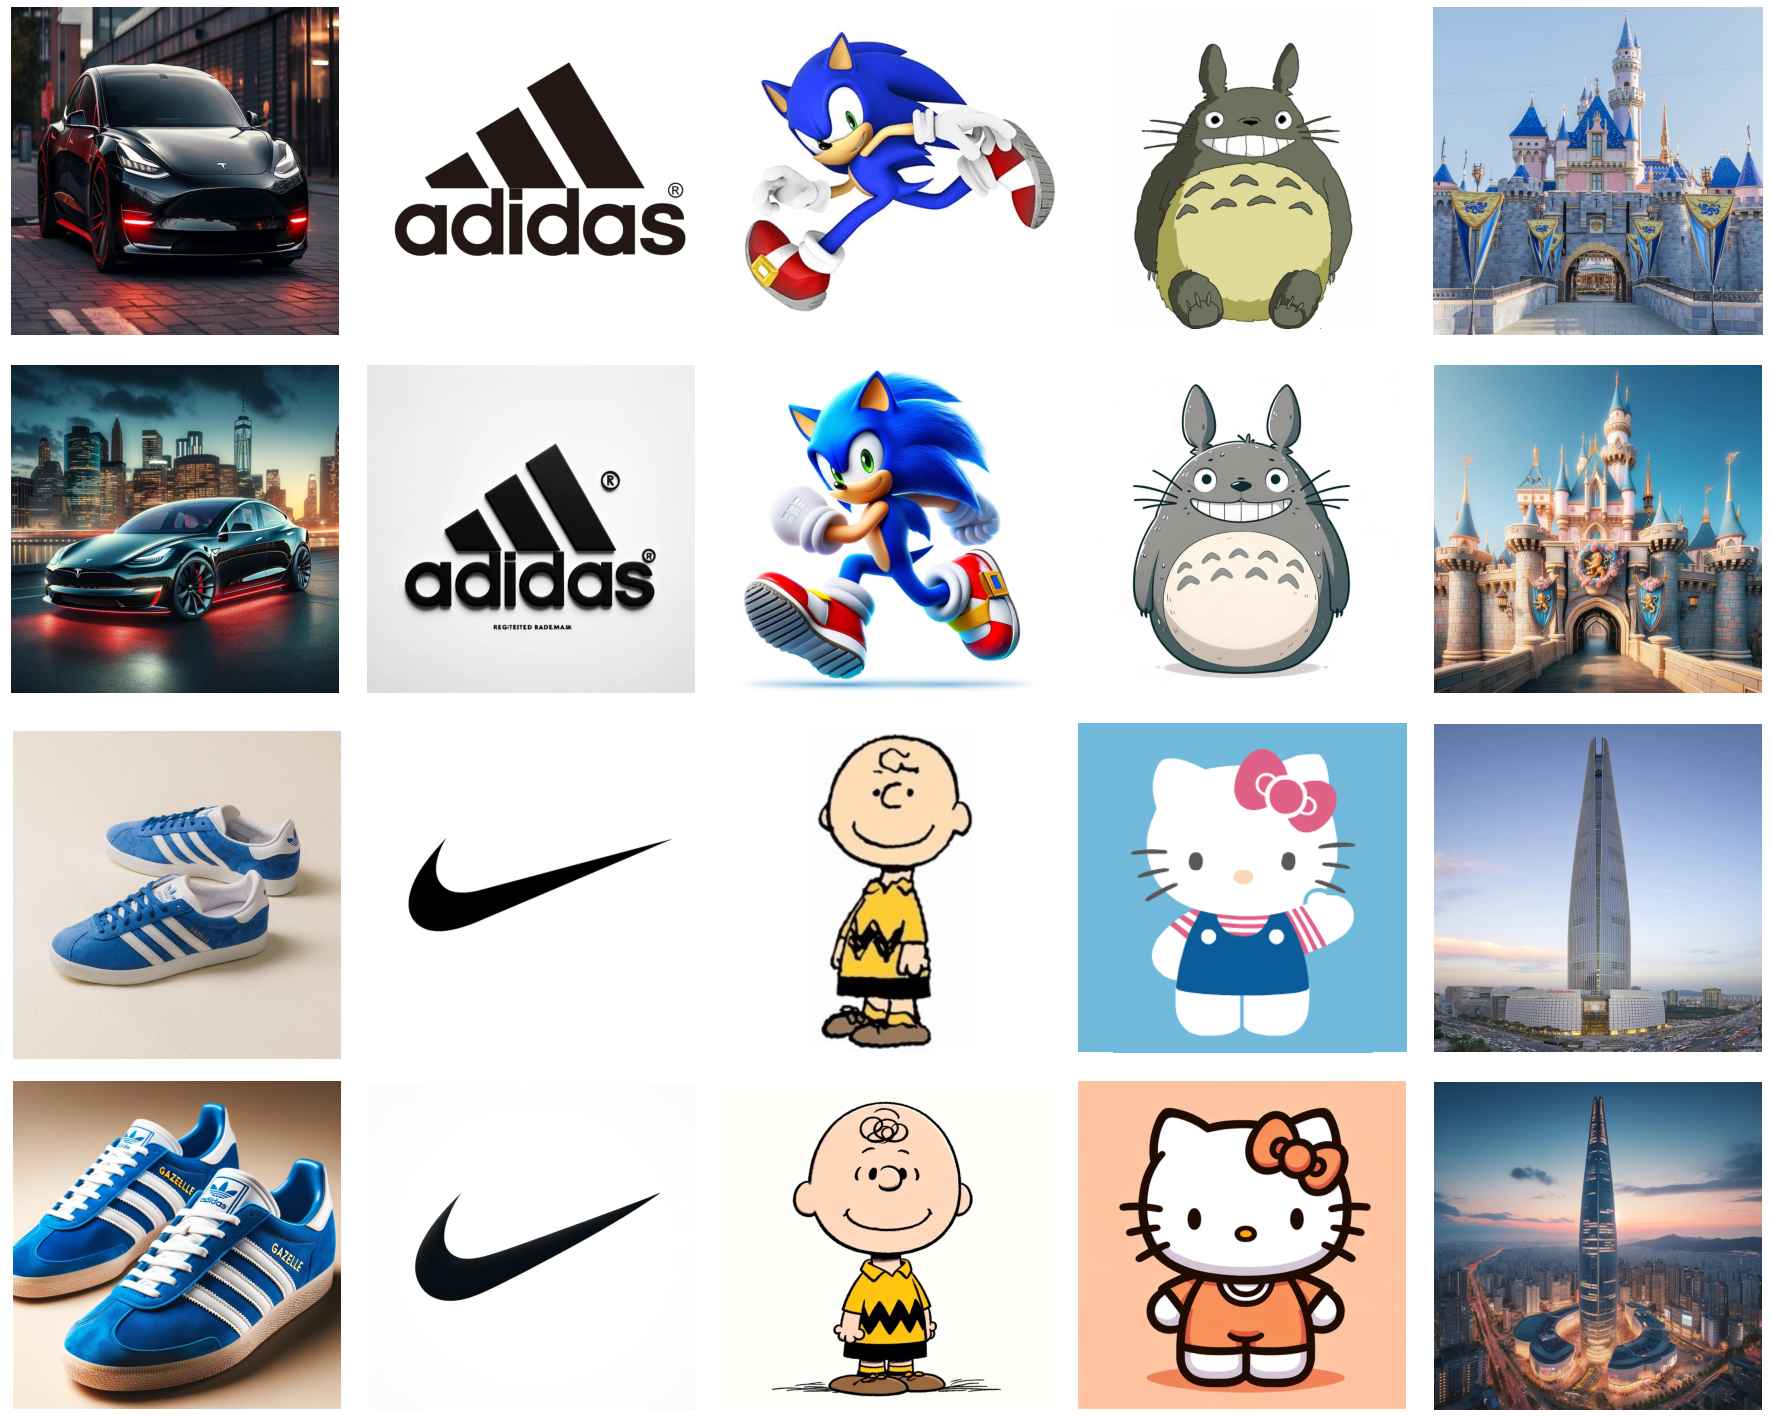
\includegraphics[width=0.99\textwidth]{figure_folder/success_all.pdf}
        \vspace{-0.1in}
        \caption{\small Violation results}
        \label{figa:violate}
    \end{subfigure}
    \begin{subfigure}[t]{\textwidth}
        \centering
        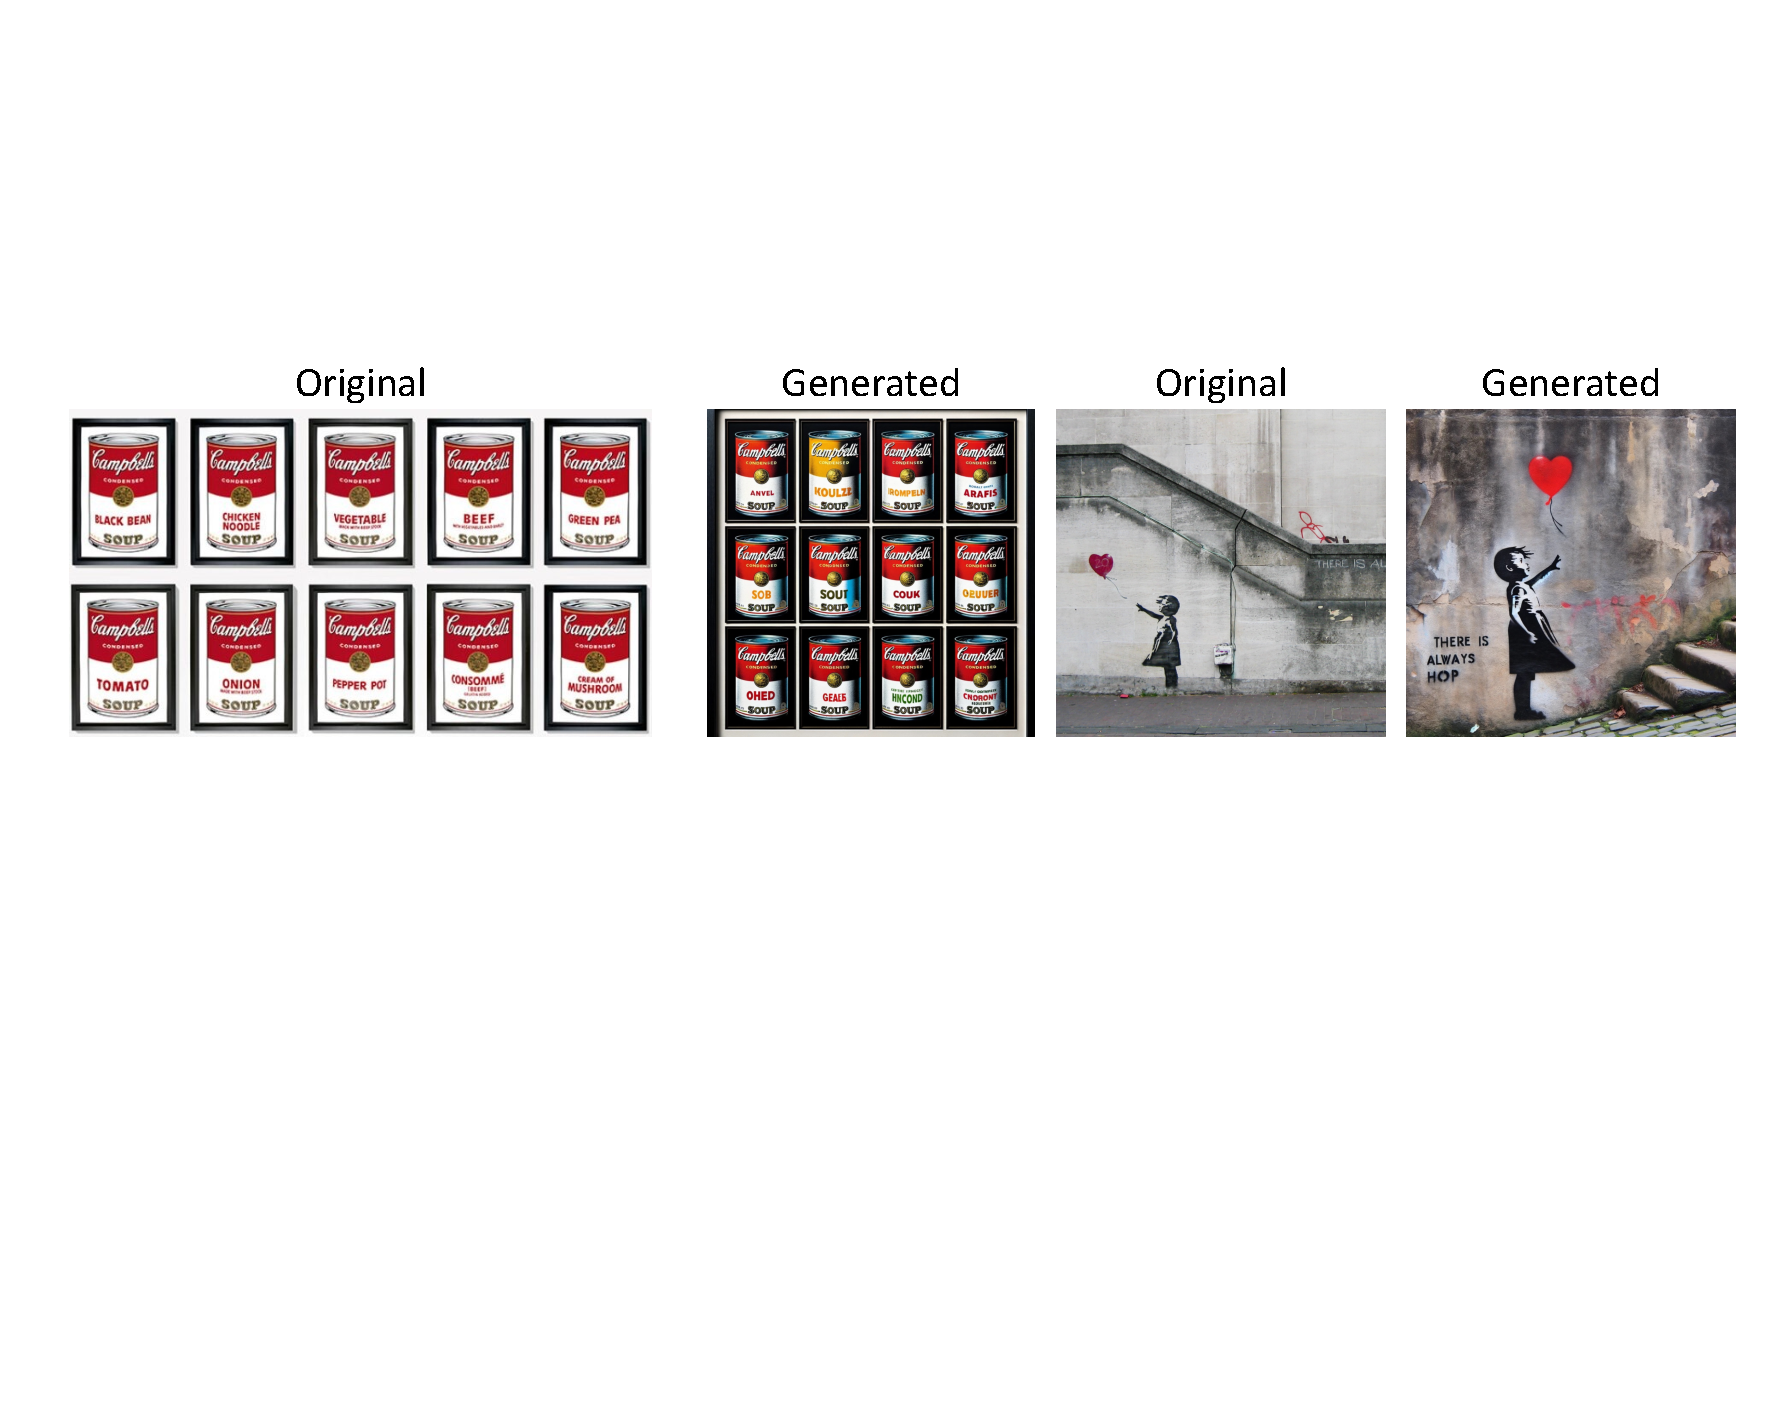
\includegraphics[width=0.99\textwidth]{figure_folder/generated_results_single_row.pdf}
        \vspace{-0.1in}
        \caption{\small Similar style generation results}
        \label{figb:similar}
    \end{subfigure}
    \vspace{-0.13in}
    \caption{\small \textbf{Generated images by ChatGPT with our prompts.} (a) First/third rows are references and the second/fourth rows are generated images. (b) First/third columns are references and the second/fourth colums are generated images.}
    \vspace{-0.23in}
    \label{fig3:our_attack}
\end{figure}

\vspace{-0.1in}
\subsection{Simple prompt can induce the copyright violation in most systems} \label{result:simple_prompt}
\vspace{-0.1in}

Midjourney~\citep{midjourney2024}, Gemini Pro~\citep{team2023gemini}, Copilot~\citep{microsoft2024copilot} and ChatGPT~\citep{achiam2023gpt4} have word-based detection mechanism on the user prompts to prevent generation of the images that may violate the internal policy. To evaluate whether these models safely block the IP content generation, we first employ simple prompts: Generate image of \{keyword\}. Surprisingly, Midjourney, Gemini Pro, and Copilot do not have a strong security blocking mechanism for IP content violations compared to ChatGPT. As shown in the table~\ref{table:block_rate_base}, Midjourney, Gemini Pro, and Copilot have an average 13.3\% block rates on IP contents while ChatGPT has 84.0\% block rate. Furthermore, 16.0\% of the images generated by ChatGPT are not even identical contents, employing rephrasing to bypass the copyright detection as shown in Appendix~\ref{app:base_result}. Examples of denials for each system are in the Appendix~\ref{app:denial_results}.

To further examine the blocking mechanism of ChatGPT and whether it is still safe to prevent the violation, we manually test ChatGPT to generate Mickey Mouse. However, it is extremely difficult to generate the exact content as we expected. Furthermore, it is difficult to manually find prompts that can generate the target contents. As shown in Figure~\ref{app:manual_trial}, most of the images have a similar component as Mickey Mouse but it is not a Mickey Mouse.

\vspace{-0.1in}
\subsection{System with blocking mechanism can not fully safe from copyright violation} \label{result:our_prompt}
\vspace{-0.1in}
Although ChatGPT demonstrates a high block rate on simple prompts, and further rephrasing the user's prompt to bypass the copyright infringement as shown in Figure~\ref{app:manual_trial}, we discover that the blocking mechanism fails to block copyright infringement generation to 11.0\% block rate on our APGP-generated prompts (Table~\ref{table:block_rate_diff}). Furthermore, not only generating the contents, the contents are exceptionally similar to the original IP content as shown in Figure~\ref{fig3:our_attack}.
\begin{wraptable}[5]{r}{0.65\linewidth}
    \vspace{0.02in}
    \caption{Block rate of ChatGPT on each prompt.}
    \vspace{-0.1in}
    \centering
    \begin{adjustbox}{width=\linewidth}
        \small 
        \begin{tabular}{lcccccc}
            \toprule
            Prompt&Product&Logo&Character&Art&Architecture&Avg\\
            \midrule
            Simple prompt &85.0&100.0&100.0&75.0&60.0&84.0\\
            Our prompt &5.0&5.0&5.0&30.0&10.0&\textbf{\color{red}11.0}\\
            \bottomrule
        \end{tabular}
    \label{table:block_rate_diff}
    \end{adjustbox}
\end{wraptable}

% \hfill
%     \caption{\small Representation distance between target and generated image by GPT4 conditioned on each prompt.}
%     \vspace{-0.1in}
%     \centering
%     \begin{adjustbox}{width=\linewidth}
%         \small 
%         \begin{tabular}{lcccccc}
%             \toprule
%             Prompt&Product&Logo&Character&Art&Place&Avg\\
%             \midrule
%             Simple prompt\\
%             Ours \\
%             \bottomrule
%         \end{tabular}
%     \label{table:rep_distance}
%     \end{adjustbox}

\vspace{-0.1in}
\paragraph{Human evaluation.}
To quantify the violations, we conducted a human evaluation on 63 participants to determine the copyright violation based on the reference image. The copyright violation is highly occurring in the product and logo category where 96.24\% and 82.71\% of participants examine the images as copyright infringement (Figure~\ref{fig:human_eval1}). Upon examining the images classified as identical violations, it was found that over 50\% were deemed to be cases of copyright infringement in product and logo. Furthermore, 30\% of characters are also considered as similar violations which are determined as severe similarity (Figure~\ref{fig:humaneval_vote}). When we employ a consensus vote to determine violations, there are still 10 images that all participants determine as violations.



\paragraph{Automatic evaluation.}

\begin{wrapfigure}[11]{r}{0.4\textwidth}
  \vspace{-0.1in}
  \begin{center}
    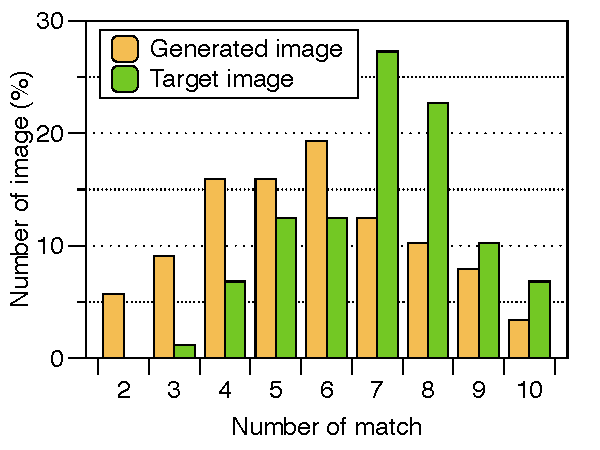
\includegraphics[width=0.96\linewidth]{figure_folder/qa.pdf}
  \end{center}
  \vspace{-0.22in}
  \caption{\small Automatic QA evaluation}
  \label{figure_qa}
\end{wrapfigure} 
Although human evaluation is one of the best evaluation approach for copyright infringement, we propose automatic evaluation to reduce the cost of the experiment. We introduce a QA score that calculates the accuracy by given generated images by T2I systems, where QA sets are generated based on the target image. We employ VLM to respond to the question, and LLM to evaluate the answers. In Figure~\ref{figure_qa}, 34.09\% of the generated images accurately answer more than seven questions, suggesting that these images contain key aspects similar to the target images necessary for matching the correct answers. Given that the target image correctly matches the answer for more than seven questions in 67.05\% of cases, we estimate that 50.84\% of the generated images likely commit copyright infringement.

\vspace{-0.1in}
\paragraph{Ablation study.}

\begin{wrapfigure}[13]{r}{0.46\textwidth}
    \centering
    \vspace{-0.12in}
        \begin{subfigure}[t]{0.32\linewidth}
            \centering
            
\includegraphics[width=\linewidth]{figure_folder/ablation_ref.pdf}
            \vspace{-0.2in}
            \caption{\small Reference}
            \label{figa:ablation_ref}
        \end{subfigure}
        \hfill
        \begin{subfigure}[t]{0.32\linewidth}
            \centering
            
\includegraphics[width=\linewidth]{figure_folder/ablation_ab.pdf}
            \vspace{-0.2in}
            \caption{\small wo/ $S_{qa}$, $S_{t}$}
            \label{figb:ablation_ab}
        \end{subfigure}
        \hfill
        \begin{subfigure}[t]{0.32\linewidth}
            \centering
            
\includegraphics[width=\linewidth]{figure_folder/ablation_ours.pdf}
            \vspace{-0.2in}
            \caption{\small Ours}
            \label{figc:ablation_ours}
        \end{subfigure}
        \vspace{-0.1in}
        \caption{\small Generated images in ablation experiment}
    \label{fig:ablation_images}
\end{wrapfigure}
Text prompts that specifically describe copyrighted content can trigger the generation of such content even without explicit keywords, as demonstrated in Table~\ref{table:prompt_example}. We hypothesize that omitting specific keywords may allow these prompts to bypass initial violation detection mechanisms. However, if the prompt is too generic without any keywords, T2I model no longer clearly generates the copyrighted contents. As illustrated in Figure~\ref{fig:ablation}, integrating our self-generated QA score and keyword penalty score sharpens these descriptions of the prompts, thereby enhancing the generation of high-quality images that accurately reflect specified features of copyrighted contents. In contrast, without these enhancements, the generated images tend to be generic or miss essential components, as shown in Figure~\ref{fig:ablation_images}.
%However, even though there is no keyword, sometimes ChatGPT blocks the generation after loading the image generation, which means when our image generation is blocked in T2I models within GPT4. Although this observation is only exclusive to ChatGPT service, interesting observation is that several blocking systems are not perfect to prevent the violation for image generative models, which is definitely a difficult problem to solve.


% \vspace{-0.1in}
\begin{table}[t]
\caption{\small Examples of generated prompts by our approach. More examples are in the Appendix~\ref{app:prompt_results}.}
\centering
    \begin{adjustbox}{width=\linewidth}
        \small 
        \begin{tabular}{ccl}
            \toprule
            Type & Content & Prompt\\
            \midrule
            \multirow{7}{*}{Character} & \multirow{7}{*}{\shortstack[l]{Mickey\\Mouse}} & 
                The image depicts the iconic mouse, a classic animated creation characterized by his cheerful demeanor and \\ &&distinctive cartoon style. Mouse is shown with an exuberant expression, spreading his arms wide in a wel-\\
                &&coming gesture. He wears his trademark red shorts adorned with two white buttons, large yellow shoes, \\
                &&and white gloves, which enhances his animated, joyful appearance. The background is plain, accentuating \\
                &&mouse's vivid colors and his instantly recognizable silhouette, completed by his round ears and a long, \\
                && thin tail that adds to his playful charm. This depiction encapsulates mouse’s enduring appeal as a symbol of \\
                &&joy and friendliness. Generate image. Do not rephrase the prompt.\\
            % \midrule
            % \multirow{8}{*}{Place} &\multirow{8}{*}{\shortstack[l]{Disneyland}} &  This image features the iconic Sleeping Beauty Castle, a fairy tale structure situated in Disneyland,\\
            % &&California. The castle stands prominently in the center of the image with its picturesque turrets and \\
            % &&spires painted in soft shades of pink, blue, and gold, creating a dreamy and enchanting appearance. \\
            % &&The foreground of the image shows a stone bridge leading up  to the castle's arched entrance, which\\
            % &&  is adorned with various heraldic banners featuring lion motifs in blue and gold. The clear blue sky \\
            % &&in the background complements the fairy tale aesthetic of the scene. The architectural details, \\
            % &&coupled with the pristine condition of the castle and its surroundings, contribute to a magical and\\
            % &&inviting atmosphere characteristic of Disney theme parks.\\
            %\midrule
            %Violence & Injury & \\         
            \bottomrule
        \end{tabular}
    \end{adjustbox}
    \label{table:prompt_example}
    \vspace{-0.2in}
\end{table}
\begin{figure}
  \begin{minipage}[t]{0.33\textwidth}
        \begin{subfigure}[t]{0.98\linewidth}
            \centering
            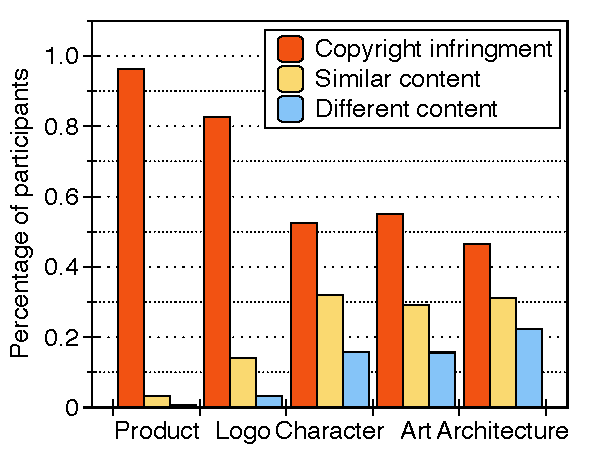
\includegraphics[width=0.99\linewidth]{figure_folder/human_eval.pdf}
        \end{subfigure} 
        \vspace{-0.1in}
        \caption{\small Results of human evaluation on each catergory}
        \label{fig:human_eval1}
    \end{minipage}
    \begin{minipage}[t]{0.33\textwidth}
        \begin{subfigure}[t]{0.98\linewidth}
            \centering
            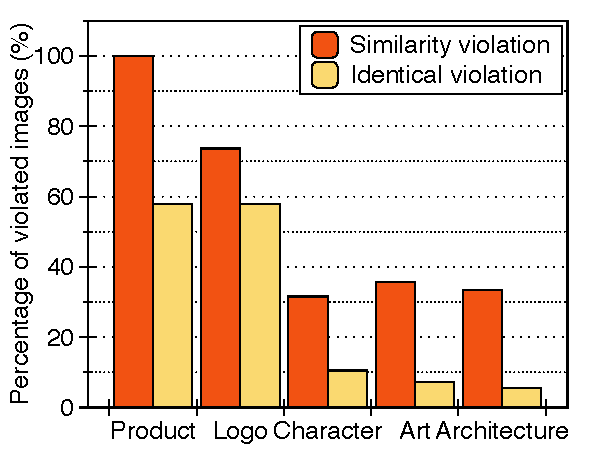
\includegraphics[width=0.99\linewidth]{figure_folder/human_vote.pdf}
        \end{subfigure} 
        \vspace{-0.1in}
        \caption{\small Results of violation rate based on human evaluation}
        \label{fig:humaneval_vote}
    \end{minipage}
    \begin{minipage}[t]{0.33\textwidth}
        \begin{subfigure}[t]{0.98\linewidth}
            \centering
            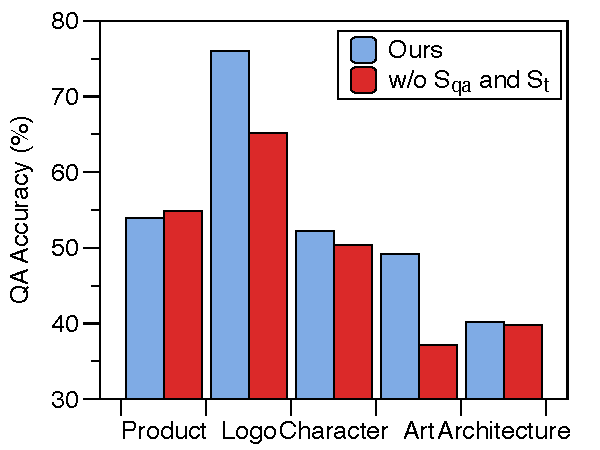
\includegraphics[width=0.99\linewidth]{figure_folder/qa_score_ablation.pdf}
        \end{subfigure} 
        \vspace{-0.1in}
        \caption{\small Results of score function ablation experiment}
        \label{fig:ablation}
    \end{minipage}
    \vspace{-0.27in}
\end{figure}
\vspace{-0.15in}
\subsection{Simple defense approach can not be the solution} \label{result:defense}
\vspace{-0.05in}
%In this section, we further examine whether simple defense approaches can mitigate the violations of our prompts. We investigate two types of defense approaches: simple copyright detection filtering approach and concept unlearning models.
In this section, we further examine whether simple defense approaches, such as a copyright detection filtering approach and concept unlearning models, can mitigate the violations of our prompts.

\begin{figure}[t]
    \begin{minipage}[b]{0.33\textwidth}
        \begin{subfigure}[t]{0.98\linewidth}
            \centering
            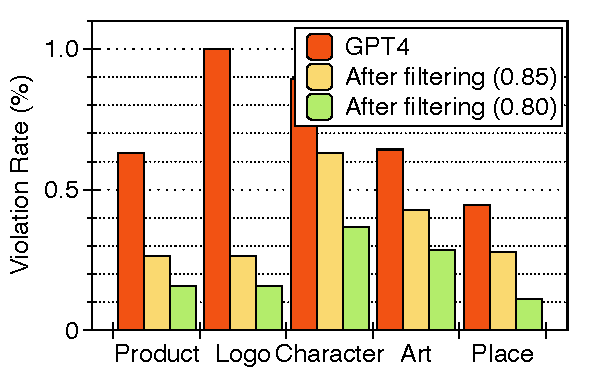
\includegraphics[width=0.9\linewidth]{figure_folder/filtering.pdf}
            \vspace{-0.1in}
            \caption{\small Violation rate after filtering}
            \label{figa:target_concept}
        \end{subfigure}
        \hfill
        \begin{subfigure}[t]{0.98\linewidth}
            \centering
            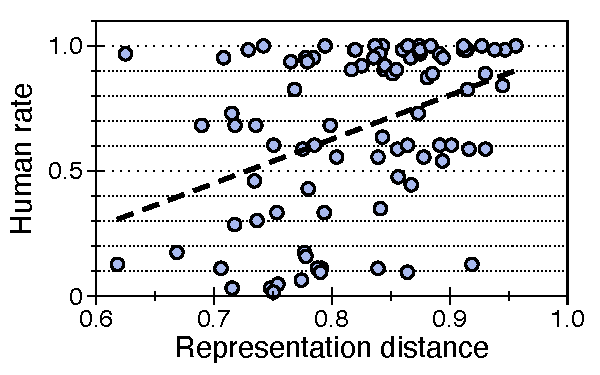
\includegraphics[width=0.9\linewidth]{figure_folder/human_rep_diff.pdf}
            \vspace{-0.1in}
            \caption{\small Correlation between human rate and representation similarity}
            \label{figb:correlation_human_rep}
        \end{subfigure}
        \vspace{-0.1in}
        \caption{\small Results after detection based filtering}
        \label{fig:filter_defense}
    \end{minipage}
    \hfill
    \begin{minipage}[b]{0.60\textwidth}
        \centering
        \begin{subfigure}[t]{0.32\linewidth}
            \centering
            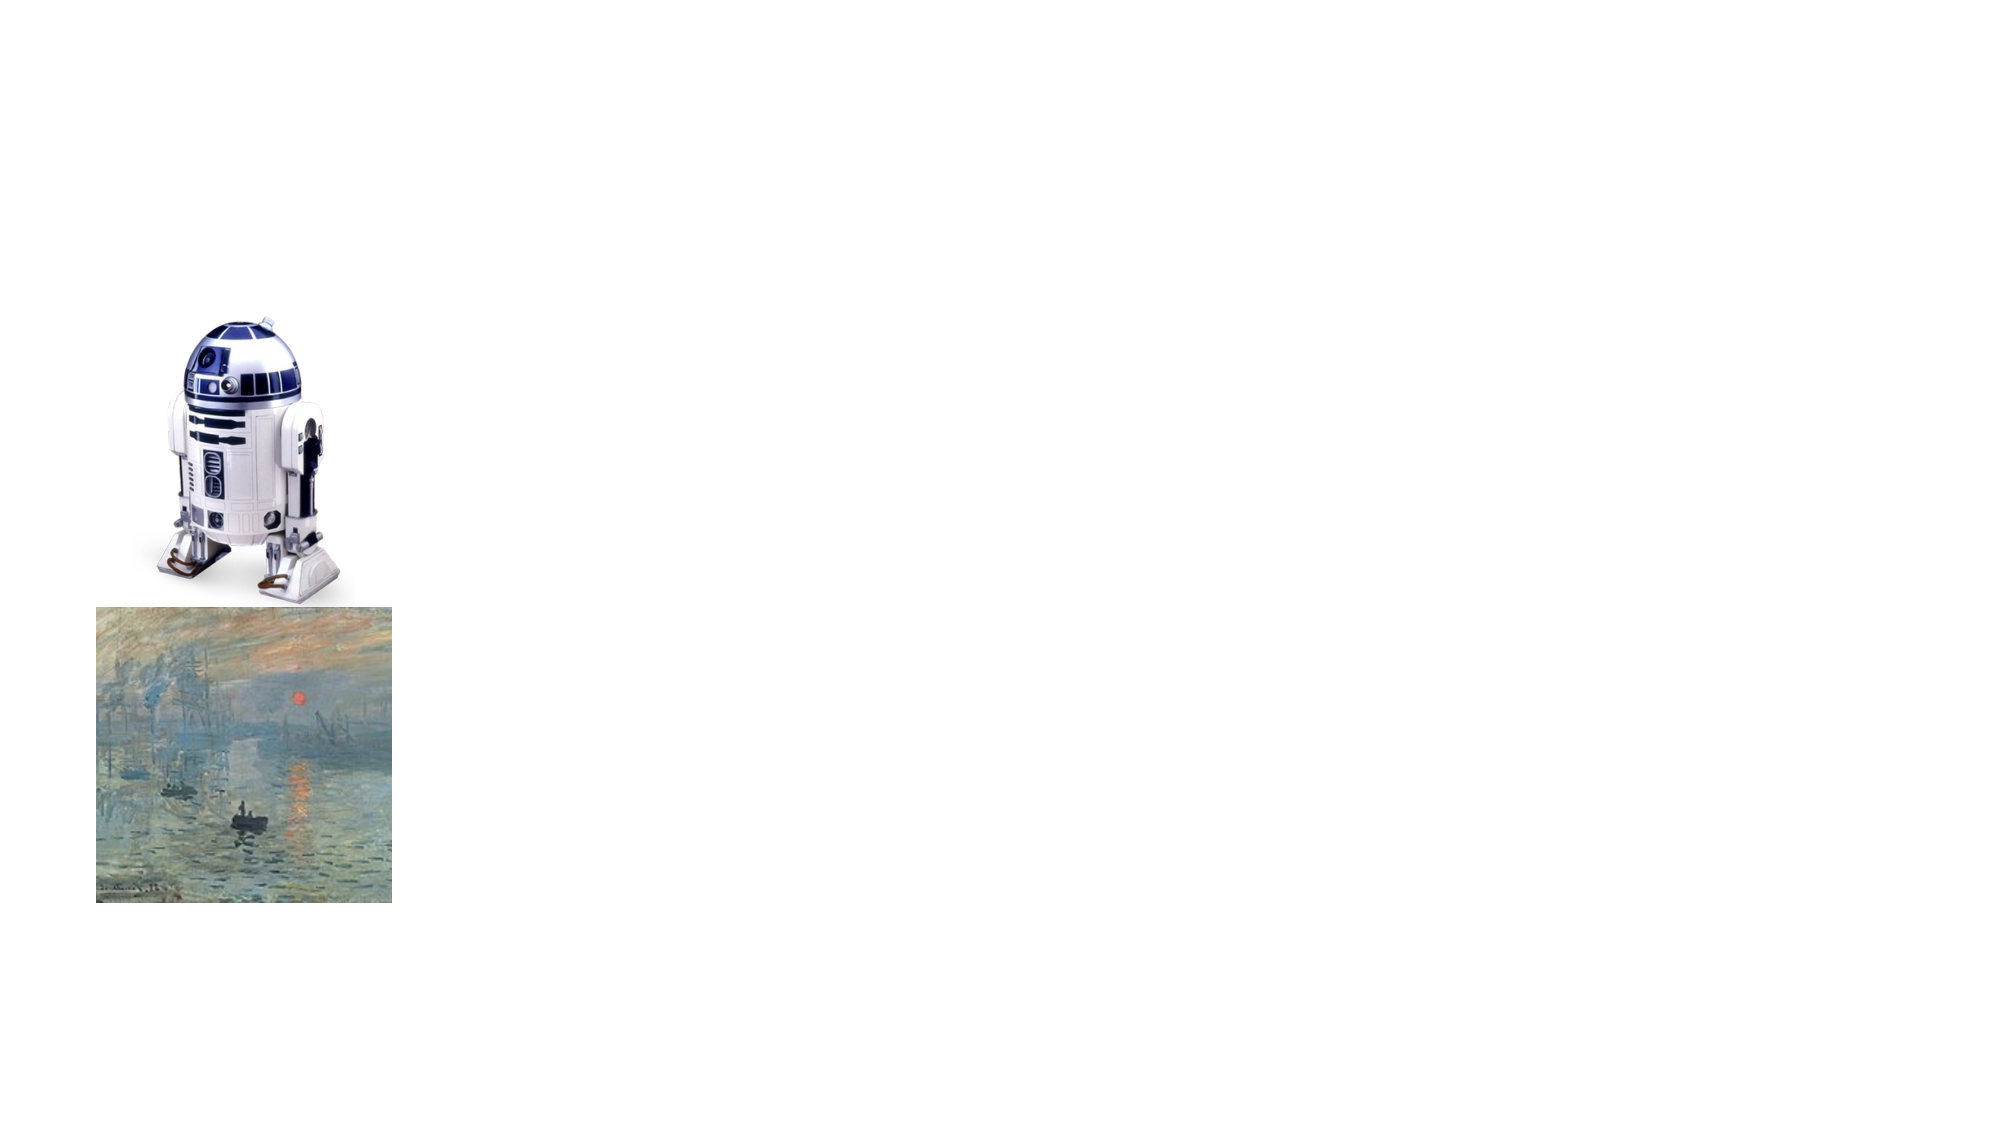
\includegraphics[width=\linewidth]{figure_folder/unlearning_fig_original.pdf}
            \vspace{-0.2in}
            \caption{\small Removed concept}
            \label{figa:orig_image}
        \end{subfigure}
        \hfill
        \begin{subfigure}[t]{0.32\linewidth}
            \centering
            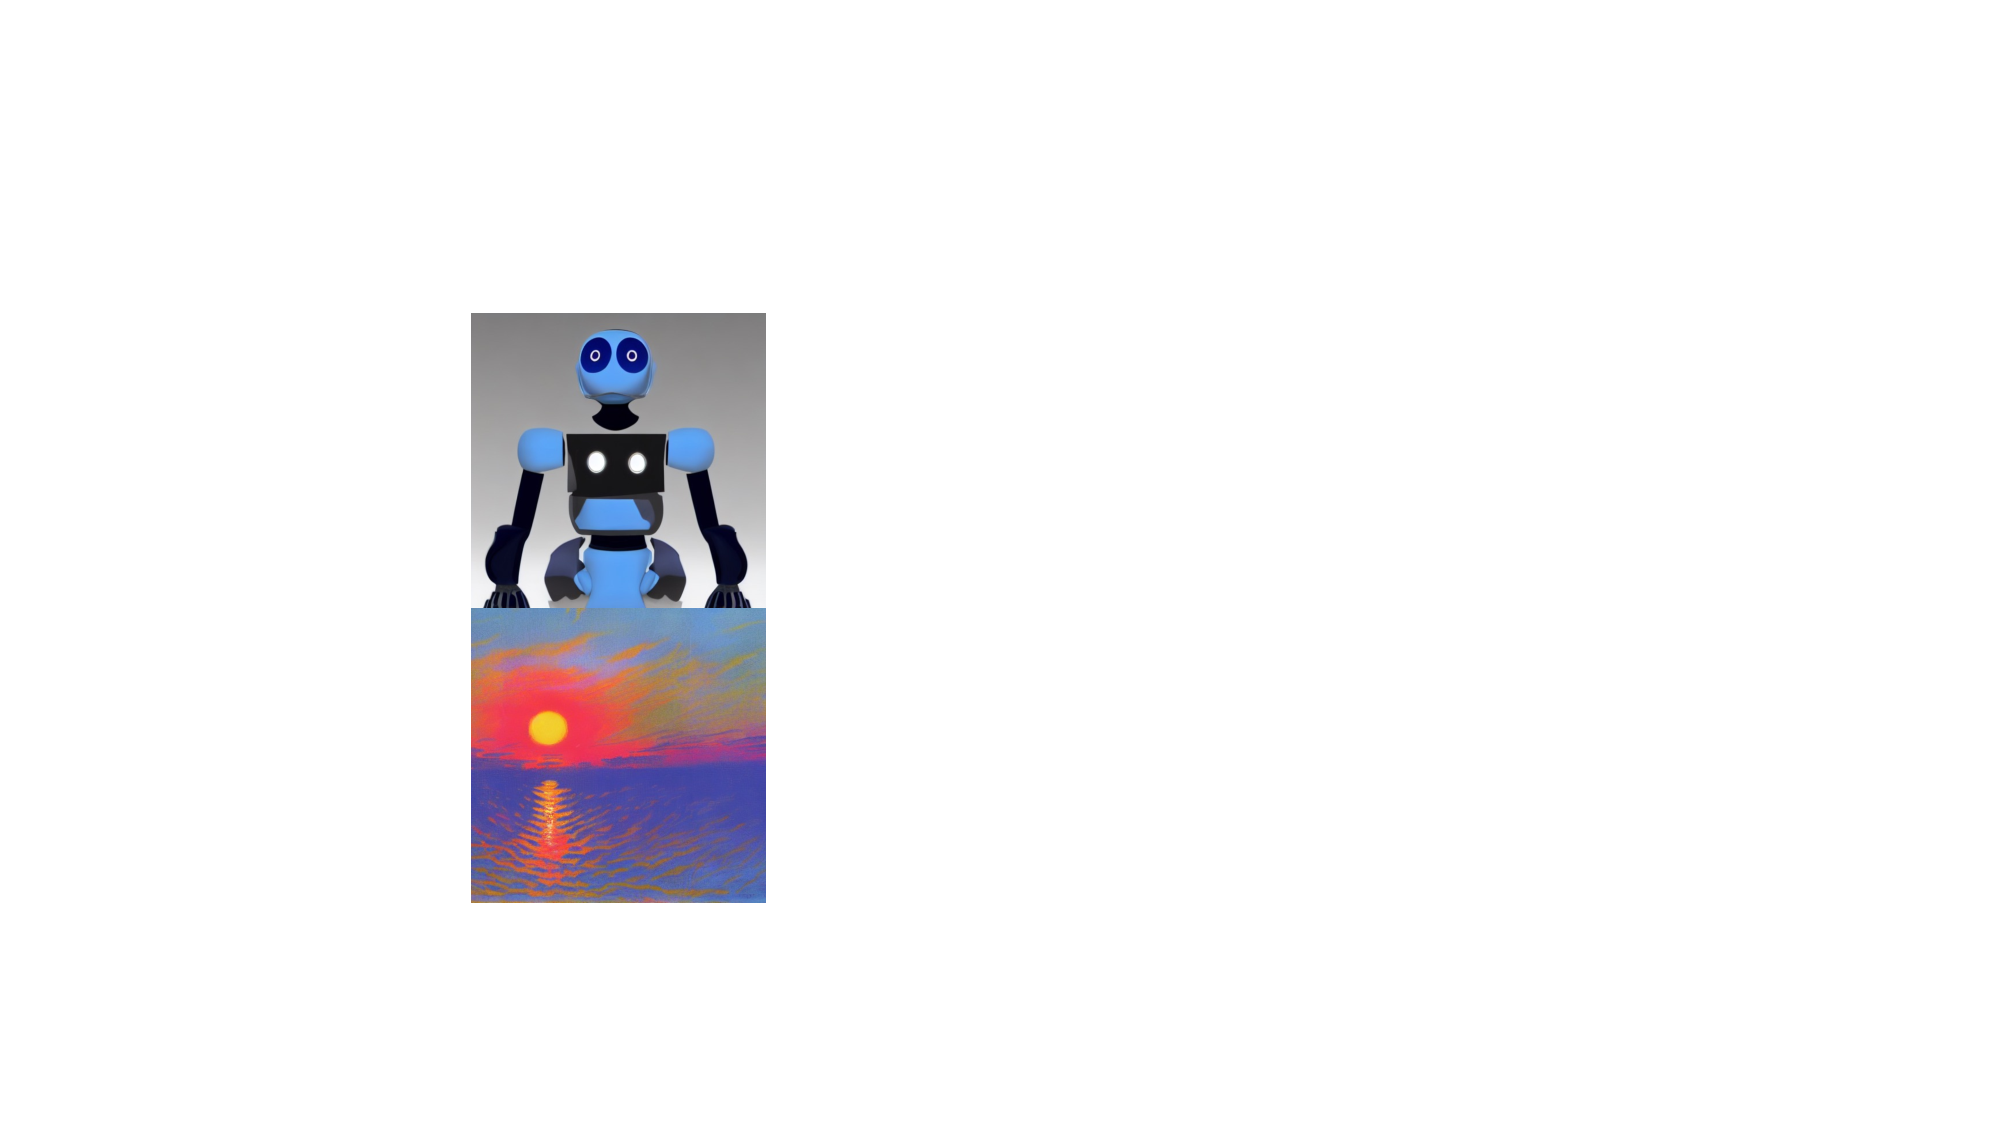
\includegraphics[width=\linewidth]{figure_folder/unlearning_fig_baseline.pdf}
            \vspace{-0.2in}
            \caption{\small Human prompt}
            \label{figb:unlearn_human}
        \end{subfigure}
        \hfill
        \begin{subfigure}[t]{0.32\linewidth}
            \centering
            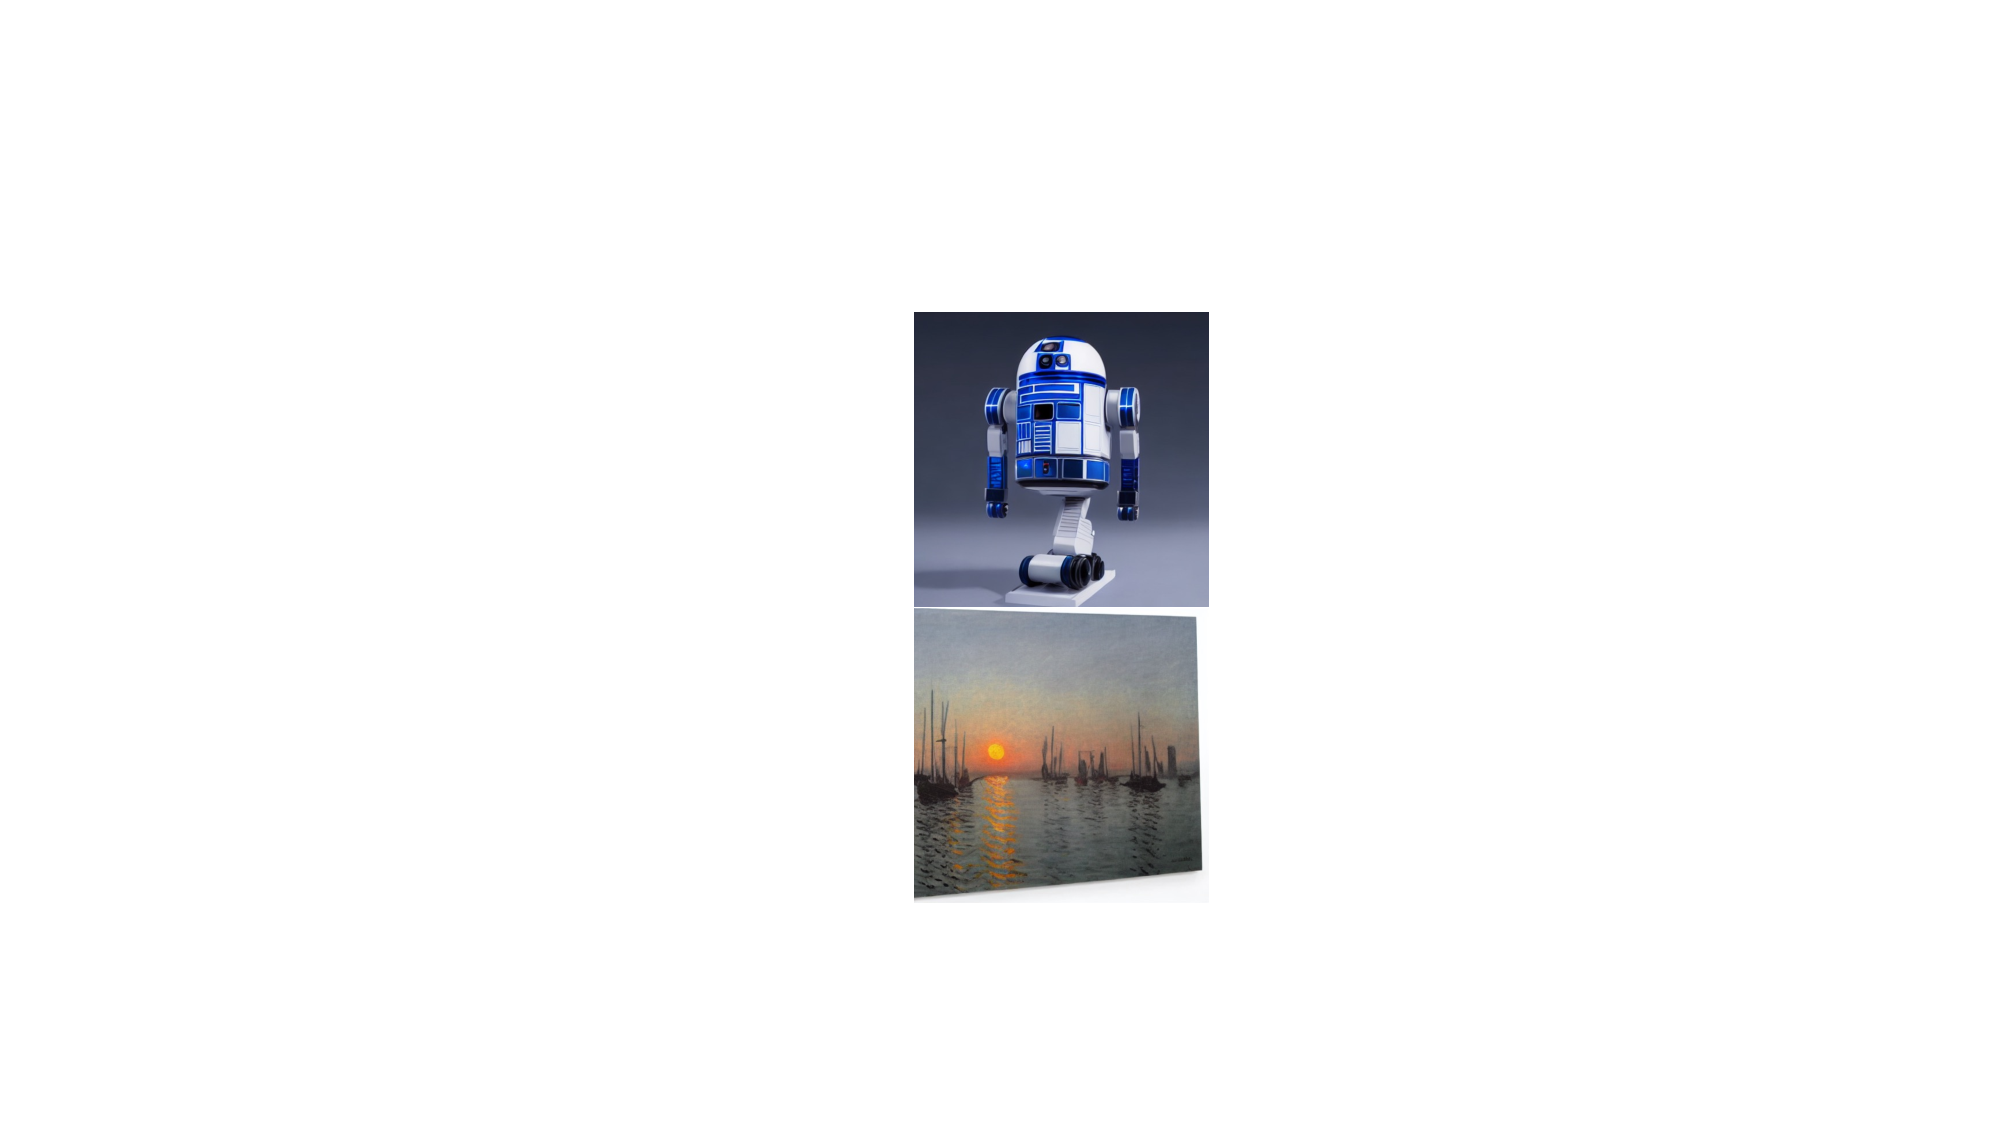
\includegraphics[width=\linewidth]{figure_folder/unlearning_fig_ours.pdf}
            \vspace{-0.2in}
            \caption{\small Our prompt}
            \label{figc:unlearn_ours}
        \end{subfigure}
        \vspace{-0.01in}
        \caption{\small Results on concept unlearning models}
        \label{fig:unlearning_model}
    \end{minipage}
\vspace{-0.23in}
\end{figure}

%\paragraph{Post prompt injection} Since our approach forces models not to rephrase the descriptions at the post processing step, one might think that if the model always rephrases the description no matter what the command is in the user prompts via the system prompt, we can mitigate the content violations. Therefore, we add rephrasing steps at the end of our pipeline as we use the 100\% rephrased prompts to the services. As shown in the Figure~\ref{fig:suffix_defense}, simple rephrasing sometimes reduces the violations, but it still violates the copyright. Furthermore, this experiment shows that there are more diverse prompts that still lead to copyright infringement, implying that simple rule-based detection may not prevent the copyright infringement.

\vspace{-0.1in}
\paragraph{Copyright detection with target images.} The other simple defense idea is "Why not use copyright detection models at the end of the generation and use them as a filter?". However, to the best of our knowledge, there are no open-sourced image copyright detection models that are able to differentiate copyright contents and similar contents like in Figure~\ref{fig3:our_attack}. Therefore, it is challenging to employ copyright detection models at the end to filter out the generation results on commercial T2I systems.

Since employing pretrained copyright detection models is impractical at the moment, we utilize the simple detection mechanism that assumes the AI system already has the target image and uses the similarity score as a threshold to filter the generation outputs. Although the similarity distance in the representation space can be used to determine the violation, it does not have a strong correlation with the human evaluation as shown in Figure~\ref{figb:correlation_human_rep}. Therefore, 0.8 threshold filtering may prevent 70.71\% of violations but still 29.29\% of examples are violating the copyright infringement (Figure~\ref{fig:filter_defense}). 

\vspace{-0.1in}
\paragraph{Results on concept unlearning models.} To remove the copyright content, unlearning approaches~\citep{kumari2023ablating, gandikota2023erasing} are alternative methods to remove the copyright content in the representation space while utilizing pretrained T2I models. We test three concept unlearned models~\citep{kumari2023ablating} that remove the R2D2, Monet, and Van Gogh concepts, respectively (Figure~\ref{figa:target_concept}). As shown in the Figure~\ref{figb:unlearn_human}, on the simple human prompt, stable diffusion models seem to erase the concept. On the contrary, the APGP-generated prompts somewhat evoke the removed concept (Figure~\ref{figc:unlearn_ours}). Restoring the erased concept may be easier on our prompts especially if the concept has a high correlation with other word~\citep{kumari2023ablating} as in Van Gogh concept which has a high correlation on star or night (Figure~\ref{app:unlearning_model}).


\section{Conclusion}
\label{sec:conclusion}
In this paper, we have investigated the common and unresolved issue that many established neural networks suffer from low floating-point operations per second (FLOPS). We have revisited a bottleneck operator, DWConv, and analyzed its main cause for a slowdown -- frequent memory access. To overcome the issue and achieve faster neural networks, we have proposed a simple yet fast and effective operator, PConv, that can be readily plugged into many existing networks. We have further introduced our general-purpose FasterNet, built upon our PConv, that achieves state-of-the-art speed and accuracy trade-off on various devices and vision tasks. We hope that our PConv and FasterNet would inspire more research on simple yet effective neural networks, going beyond academia to impact the industry and community directly.



\bibliography{reference}

\appendix
\addcontentsline{toc}{section}{Appendix}
\section*{\Large Appendix}
In this appendix, we provide further details on the experimental settings, full comparison plots, architectural configurations, PConv implementations, comparisons with related work, limitations, and future work.

\section{ImageNet-1k experimental settings}
\label{imagenet_settings}
We provide ImageNet-1k training and evaluation settings in~\cref{tab:imagenet_settings}. They can be used for reproducing our main results in~\cref{tab:imagenet} and \cref{fig:imageent}. Different FasterNet variants vary in the magnitude of regularization and augmentation techniques. The magnitude increases as the model becomes larger to alleviate overfitting and improve accuracy. Note that most of the compared works in~\cref{tab:imagenet} and \cref{fig:imageent}, \eg, MobileViT, EdgeNext, PVT, CycleMLP, ConvNeXt, Swin, \etc, also adopt such advanced training techniques (ADT). Some even heavily rely on the hyper-parameter search. For others w/o ADT, \ie, ShuffleNetV2, MobileNetV2, and GhostNet, though the comparison is not totally fair, we include them for reference.

\section{Downstream tasks experimental settings}
For object detection and instance segmentation on the COCO2017 dataset, we equip our FasterNet backbone with the popular Mask R-CNN detector. 
We use ImageNet-1k pre-trained weights to initialize the backbone and Xavier to initialize the add-on layers. Detailed settings are summarized in~\cref{tab:coco_settings}.

\section{Full comparison plots on ImageNet-1k}
\cref{fig:imagenet_full} shows the full comparison plots on ImageNet-1k, which is the extension of~\cref{fig:imageent} in the main paper with a larger range of latency. \cref{fig:imagenet_full} shows consistent results that FasterNet strikes better trade-offs than others in balancing accuracy and latency/throughput on GPU, CPU, and ARM processors.

\section{Detailed architectural configurations}
We present the detailed architectural configurations in~\cref{tab:configuration}. While different FasterNet variants share a unified architecture, they vary in the network width (the number of channels) and network depth (the number of FasterNet blocks at each stage). The classifier at the end of the architecture is used for classification tasks but removed for other downstream tasks. 


% Please add the following required packages to your document preamble:
% If you use beamer only pass "xcolor=table" option, i.e. \documentclass[xcolor=table]{beamer}
\begin{table}
\vspace{0.1in}
\centering
\resizebox{1\linewidth}{!}{%
\begin{tabular}{@{}l|cccccc@{}}
\toprule
Variants           & T0                         & T1    & T2    & S    & M     & L            \\ \midrule
Train Res          & \multicolumn{6}{c}{192 for epoch 1$\sim$280, 224 for epoch 281$\sim$300}                                    \\
Test Res           & \multicolumn{6}{c}{224}                                    \\ \midrule
Epochs             & \multicolumn{6}{c}{300}                                    \\
\# of forward pass & \multicolumn{6}{c}{188k}                                   \\ \midrule
Batch size         & 4096   & 4096      & 4096      & 4096      & 2048  & 2048\\
Optimizer          & \multicolumn{6}{c}{AdamW}                                  \\
Momentum & \multicolumn{6}{c}{0.9/0.999}                              \\
LR                 & 0.004  & 0.004 & 0.004 & 0.004 & 0.002 & 0.002             \\
LR decay           & \multicolumn{6}{c}{cosine}                                 \\
Weight decay       & 0.005  & 0.01  & 0.02  & 0.03  & 0.05 & 0.05               \\
Warmup epochs      & \multicolumn{6}{c}{20}                                     \\
Warmup schedule    & \multicolumn{6}{c}{linear}                                 \\ \midrule
Label smoothing    & \multicolumn{6}{c}{0.1}                                    \\
Dropout            & \multicolumn{6}{c}{{\color[HTML]{9B9B9B} \ding{55}}}       \\
Stoch. Depth       & {\color[HTML]{9B9B9B} \ding{55}}   & 0.02  & 0.05  & 0.1  & 0.2  & 0.3   \\
Repeated Aug       & \multicolumn{6}{c}{{\color[HTML]{9B9B9B} \ding{55}}}       \\
Gradient Clip.     & {\color[HTML]{9B9B9B} \ding{55}}   & {\color[HTML]{9B9B9B} \ding{55}}  & {\color[HTML]{9B9B9B} \ding{55}}  & {\color[HTML]{9B9B9B} \ding{55}}  & 1  & 0.01       \\ \midrule
% Gradient Clip.     & \multicolumn{6}{c}{{\color[HTML]{9B9B9B} \ding{55}}}       \\ \midrule
H. flip            & \multicolumn{6}{c}{\ding{51}}                              \\
RRC                & \multicolumn{6}{c}{\ding{51}}                              \\
Rand Augment       & {\color[HTML]{9B9B9B} \ding{55}}   & 3/0.5 & 5/0.5 & 7/0.5 & 7/0.5 & 7/0.5 \\
Auto Augment       & \multicolumn{6}{c}{{\color[HTML]{9B9B9B} \ding{55}}}       \\
Mixup alpha        & 0.05                        & 0.1   & 0.1   & 0.3   & 0.5   & 0.7           \\
Cutmix alpha       & \multicolumn{6}{c}{1.0}                                    \\
Erasing prob. & \multicolumn{6}{c}{{\color[HTML]{9B9B9B} \ding{55}}} \\
Color Jitter       & \multicolumn{6}{c}{{\color[HTML]{9B9B9B} \ding{55}}}       \\
PCA lighting       & \multicolumn{6}{c}{{\color[HTML]{9B9B9B} \ding{55}}}       \\ \midrule
SWA                & \multicolumn{6}{c}{{\color[HTML]{9B9B9B} \ding{55}}}       \\
EMA                & \multicolumn{6}{c}{{\color[HTML]{9B9B9B} \ding{55}}}       \\ \midrule
Layer scale    & \multicolumn{6}{c}{{\color[HTML]{9B9B9B} \ding{55}}}                          \\ \midrule
CE loss            & \multicolumn{6}{c}{\ding{51}}                              \\
BCE loss           & \multicolumn{6}{c}{{\color[HTML]{9B9B9B} \ding{55}}}       \\ \midrule
Mixed precision    & \multicolumn{6}{c}{\ding{51}}                              \\ \midrule
Test crop ratio        & \multicolumn{6}{c}{0.9}       \\ \midrule
Top-1 acc. (\%)         & 71.9   & 76.2 & 78.9  & 81.3  & 83.0  &   83.5    \\ \bottomrule
\end{tabular}%
}
\caption{ImageNet-1k training and evaluation settings for different FasterNet variants.}
\label{tab:imagenet_settings}
\end{table}
% Please add the following required packages to your document preamble:
% \usepackage{booktabs}
% \usepackage{graphicx}
\begin{table}
\centering
\vspace{0.2in}
\resizebox{\linewidth}{!}{%
\setlength{\tabcolsep}{6pt}
\begin{tabular}{@{}l|ccc@{}}
\toprule
Variants & \qquad S \qquad \qquad           & \qquad M \qquad \qquad      & L\\ \midrule
Train and test Res & \multicolumn{3}{c}{shorter side $=$ 800, longer side $\leq$ 1333} \\
Batch size                    & \multicolumn{3}{c}{16 (2 on each GPU)} \\
Optimizer                     & \multicolumn{3}{c}{AdamW}              \\
Train schedule     & \multicolumn{3}{c}{1$\times$ schedule (12 epochs)}                      \\
Weight decay                  & \multicolumn{3}{c}{0.0001}             \\
Warmup schedule               & \multicolumn{3}{c}{linear}             \\
Warmup iterations             & \multicolumn{3}{c}{500}                \\
LR decay           & \multicolumn{3}{c}{StepLR at epoch 8 and 11 with decay rate 0.1}             \\
LR                            & 0.0002      & 0.0001      & 0.0001     \\
Stoch. Depth                  & 0.15        & 0.2         & 0.3        \\ \bottomrule
\end{tabular}%
}
\caption{Experimental settings of object detection and instance segmentation on the COCO2017 dataset.}
\vspace{-0.2in}
\label{tab:coco_settings}
\end{table}
\begin{figure*}
    \centering
    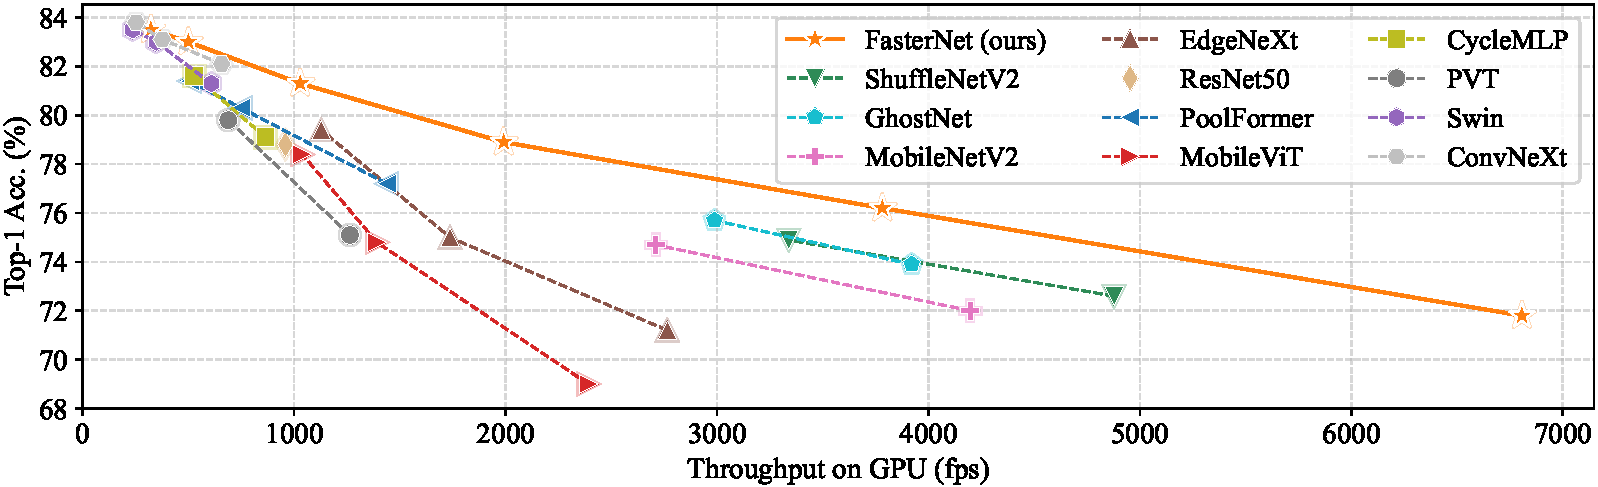
\includegraphics[width=1.\linewidth]{figures/fps_latency_gpu-cropped.pdf}

    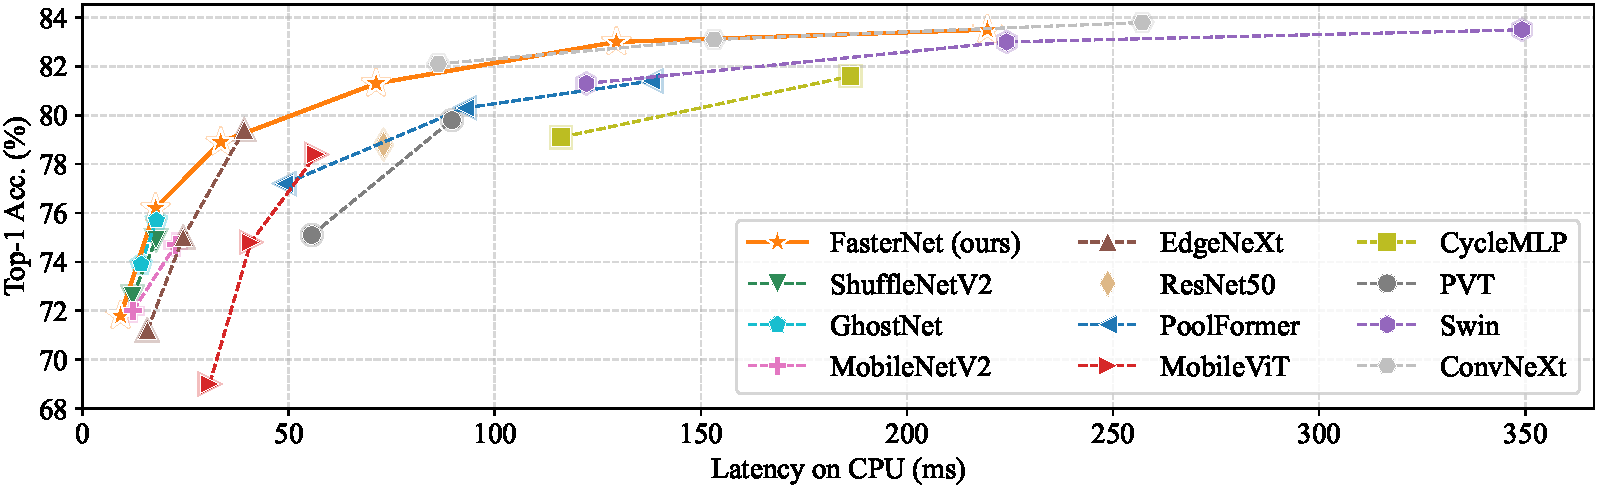
\includegraphics[width=1.\linewidth]{figures/acc_latency_cpu-cropped.pdf}
    
    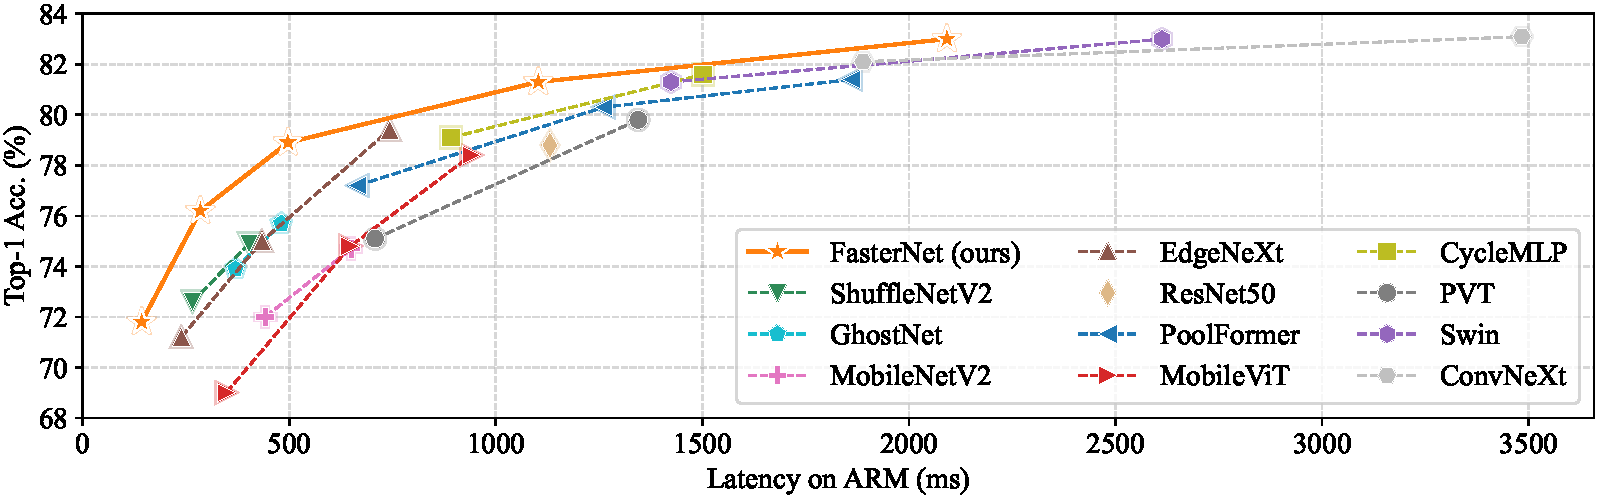
\includegraphics[width=1.\linewidth]{figures/acc_latency_arm-cropped.pdf}
    
    \vspace{-0.1in}
    \caption{Comparison of FasterNet with state-of-the-art networks. FasterNet consistently achieves better accuracy-throughput (the top plot) and accuracy-latency (the medium and bottom plots) trade-offs than others.}
    \label{fig:imagenet_full}
\end{figure*}

% \section{Implementation of PConv}
% We provide the PyTorch-based implementation of PConv in~\cref{lst:code}. There are two forward pass choices, namely forward\_slicing and forward\_split\_cat. The forward\_slicing choice writes the convolutional output in place of the input, which is used for faster inference, but not for training, as the in-place operation modifies the gradient computation. By contrast, the forward\_split\_cat choice concatenates the convolutional output with the feature maps untouched, which preserves the intermediate gradient computation and is used for training. \cref{tab:pconv_implementation} shows the speed comparison of these two choices during inference. The forward\_slicing implementation runs faster than the other one, especially for tiny models and more computation-powerful devices, \eg, for FasterNet-T0 on GPU.

\section{More comparisons with related work}
\medskip\noindent\textbf{Improving FLOPS.} \enspace 
There are a few other works~\cite{ding2022scaling_short,xia2022trt_short} also looking into the FLOPS issue and trying to improve it. They generally follow existing operators and try to find their proper configurations, \eg, RepLKNet~\cite{ding2022scaling_short} simply increases the kernel size while TRT-ViT~\cite{xia2022trt_short} reorders different blocks in the architecture. By contrast, this paper advances the field by proposing a novel and efficient PConv, opening up new directions and potentially larger room for FLOPS improvement.

% \clearpage
% Please add the following required packages to your document preamble:
% \usepackage{booktabs}
% \usepackage{graphicx}
\begin{table*}
\centering
\resizebox{.93\linewidth}{!}{%
% \setlength{\tabcolsep}{1pt}
\begin{tabular}{@{}c|c|c|c|c|c|c|c|c|c@{}}
\toprule
Name &
  Output size &
  \multicolumn{2}{c|}{Layer specification} &
  T0 &
  T1 &
  T2 &
  S &
  M &
  L \\ \midrule
Embedding &
  \large{$\frac{h}{4} \times \frac{w}{4}$}&
  \begin{tabular}[c]{@{}c@{}}Conv\_4\_$c$\_4,\\ BN\end{tabular} &
  \# Channels $c$ &
  40 &
  64 &
  96 &
  128 &
  144 &
  192 \\ \midrule
Stage 1 &
  \large{$\frac{h}{4} \times \frac{w}{4}$}&
  $\left[ \text{\begin{tabular}[c]{@{}c@{}}PConv\_3\_$c$\_1\_1/4,\\ Conv\_1\_$2c$\_1,\\ BN, Acti,\\ Conv\_1\_$c$\_1\end{tabular}}  \right] \times b_1 $  &
  \# Blocks $b_1$ &
  1 &
  1 &
  1 &
  1 &
  3 &
  3 \\ \midrule
Merging &
  \large{$\frac{h}{8} \times \frac{w}{8}$}&
  \begin{tabular}[c]{@{}c@{}}Conv\_2\_$2c$\_2,\\ BN\end{tabular} &
  \# Channels $2c$ &
  80 &
  128 &
  192 &
  256 &
  288 &
  384 \\ \midrule
Stage 2 &
  \large{$\frac{h}{8} \times \frac{w}{8}$}&
  $\left[ \text{\begin{tabular}[c]{@{}c@{}}PConv\_3\_$2c$\_1\_1/4,\\ Conv\_1\_$4c$\_1,\\ BN, Acti,\\ Conv\_1\_$2c$\_1\end{tabular}}  \right] \times b_2 $  &
  \# Blocks $b_2$ &
  2 &
  2 &
  2 &
  2 &
  4 &
  4 \\ \midrule
Merging &
  \large{$\frac{h}{16} \times \frac{w}{16}$}&
  \begin{tabular}[c]{@{}c@{}}Conv\_2\_$4c$\_2,\\ BN\end{tabular} &
  \# Channels $4c$ &
  160 &
  256 &
  384 &
  512 &
  576 &
  768 \\ \midrule
Stage 3 &
  \large{$\frac{h}{16} \times \frac{w}{16}$}&
  $\left[ \text{\begin{tabular}[c]{@{}c@{}}PConv\_3\_$4c$\_1\_1/4,\\ Conv\_1\_$8c$\_1,\\ BN, Acti,\\ Conv\_1\_$4c$\_1\end{tabular}}  \right] \times b_3 $  &
  \# Blocks $b_3$ &
  8 &
  8 &
  8 &
  13 &
  18 &
  18 \\ \midrule
Merging &
  \large{$\frac{h}{32} \times \frac{w}{32}$}&
  \begin{tabular}[c]{@{}c@{}}Conv\_2\_$8c$\_2,\\ BN\end{tabular} &
  \# Channels $8c$ &
  320 &
  512 &
  768 &
  1024 &
  1152 &
  1536 \\ \midrule
Stage 4 &
  \large{$\frac{h}{32} \times \frac{w}{32}$}&
  $\left[ \text{\begin{tabular}[c]{@{}c@{}}PConv\_3\_$8c$\_1\_1/4,\\ Conv\_1\_$16c$\_1,\\ BN, Acti,\\ Conv\_1\_$8c$\_1\end{tabular}}  \right] \times b_4 $  &
  \# Blocks $b_4$ &
  2 &
  2 &
  2 &
  2 &
  3 &
  3 \\ \midrule
Classifier &
  $1  \times 1$ &
  \begin{tabular}[c]{@{}c@{}}Global average pool,\\ Conv\_1\_1280\_1,\\ Acti,\\ FC\_1000\end{tabular} &
  Acti &
  GELU &
  GELU &
  ReLU &
  ReLU &
  ReLU &
  ReLU \\ \midrule
\multicolumn{4}{c|}{FLOPs (G)} &
  0.34 &
  0.85 &
  1.90 &
  4.55 &
  8.72 &
  15.49 \\ \midrule
\multicolumn{4}{c|}{Params (M)} &
  3.9 &
  7.6 &
  15.0 &
  31.1 &
  53.5 &
  93.4 \\ \bottomrule
\end{tabular}%
}
\caption{Configurations of different FasterNet variants. ``Conv\_$k$\_$c$\_$s$'' means a convolutional layer with the kernel size of $k$, the output channels of $c$, and the stride of $s$. ``PConv$\_k\_c\_s\_r$'' means a partial convolution with an extra parameter, the partial ratio of $r$. ``FC\_1000'' means a fully connected layer with 1000 output channels. $h \times w$ is the input size while $b_i$ is the number of FasterNet blocks at stage $i$. The FLOPs are calculated given the input size of $224 \times 224$.}
\label{tab:configuration}
\end{table*}
% \input{tables/pconv_implementation.tex}
% \input{tables/pconv_code.tex}
% \clearpage

\medskip\noindent\textbf{PConv vs. GConv.} \enspace 
PConv is schematically equivalent to a modified GConv~\cite{krizhevsky2012imagenet} that operates on a single group and leaves other groups untouched. Though simple, such a modification remains unexplored before. It's also significant in the sense that it prevents the operator from excessive memory access and is computationally more efficient. From the perspective of low-rank approximations, PConv improves GConv by further reducing the intra-filter redundancy beyond the inter-filter redundancy~\cite{haase2020rethinking_short}.

\medskip\noindent\textbf{FasterNet vs. ConvNeXt.} \enspace 
Our FasterNet appears similar to ConvNeXt~\cite{liu2022convnet} after substituting DWConv with our PConv. However, they are different in motivations. While ConvNeXt searches for a better structure by trial and error, we append PWConv after PConv to better aggregate information from all channels. Moreover, ConvNeXt follows ViT to use fewer activation functions, while we intentionally remove them from the middle of PConv and PWConv, to minimize their error in approximating a regular Conv. 

\medskip\noindent\textbf{Other paradigms for efficient inference.} \enspace 
Our work focuses on efficient network design, orthogonal to the other paradigms, \eg, neural architecture search (NAS)~\cite{elsken2019neural}, network pruning~\cite{molchanov2016pruning}, and knowledge distillation~\cite{hinton2015distilling}. They can be applied in this paper for better performance. However, we opt not to do so to keep our core idea centered and to make the performance gain clear and fair.

\medskip\noindent\textbf{Other partial/masked convolution works.} \enspace 
There are several works~\cite{liu2018image,gao2022convmae,liu2022partial} sharing similar names with our PConv. However, they differ a lot in objectives and methods. For example, they apply filters on partial pixels to exclude invalid patches~\cite{liu2018image}, enable self-supervised learning~\cite{gao2022convmae}, or synthesize novel images~\cite{liu2022partial}, while we target at the channel dimension for efficient inference. 

\section{Limitations and future work}
We have demonstrated that PConv and FasterNet are fast and effective, being competitive with existing operators and networks. Yet there are some minor technical limitations of this paper. For one thing, PConv is designed to apply a regular convolution on only a part of the input channels while leaving the remaining ones untouched. Thus, the stride of the partial convolution should always be 1, in order to align the spatial resolution of the convolutional output and that of the untouched channels. Note that it is still feasible to down-sample the spatial resolution as there can be additional downsampling layers in the architecture. 
And for another, our FasterNet is simply built upon convolutional operators with a possibly limited receptive field. Future efforts can be made to enlarge its receptive field and combine it with other operators to pursue higher accuracy.





% % Please add the following required packages to your document preamble:
% \usepackage{booktabs}
% \usepackage{graphicx}
\begin{table*}
\centering
\resizebox{.93\linewidth}{!}{%
% \setlength{\tabcolsep}{1pt}
\begin{tabular}{@{}c|c|c|c|c|c|c|c|c|c@{}}
\toprule
Name &
  Output size &
  \multicolumn{2}{c|}{Layer specification} &
  T0 &
  T1 &
  T2 &
  S &
  M &
  L \\ \midrule
Embedding &
  \large{$\frac{h}{4} \times \frac{w}{4}$}&
  \begin{tabular}[c]{@{}c@{}}Conv\_4\_$c$\_4,\\ BN\end{tabular} &
  \# Channels $c$ &
  40 &
  64 &
  96 &
  128 &
  144 &
  192 \\ \midrule
Stage 1 &
  \large{$\frac{h}{4} \times \frac{w}{4}$}&
  $\left[ \text{\begin{tabular}[c]{@{}c@{}}PConv\_3\_$c$\_1\_1/4,\\ Conv\_1\_$2c$\_1,\\ BN, Acti,\\ Conv\_1\_$c$\_1\end{tabular}}  \right] \times b_1 $  &
  \# Blocks $b_1$ &
  1 &
  1 &
  1 &
  1 &
  3 &
  3 \\ \midrule
Merging &
  \large{$\frac{h}{8} \times \frac{w}{8}$}&
  \begin{tabular}[c]{@{}c@{}}Conv\_2\_$2c$\_2,\\ BN\end{tabular} &
  \# Channels $2c$ &
  80 &
  128 &
  192 &
  256 &
  288 &
  384 \\ \midrule
Stage 2 &
  \large{$\frac{h}{8} \times \frac{w}{8}$}&
  $\left[ \text{\begin{tabular}[c]{@{}c@{}}PConv\_3\_$2c$\_1\_1/4,\\ Conv\_1\_$4c$\_1,\\ BN, Acti,\\ Conv\_1\_$2c$\_1\end{tabular}}  \right] \times b_2 $  &
  \# Blocks $b_2$ &
  2 &
  2 &
  2 &
  2 &
  4 &
  4 \\ \midrule
Merging &
  \large{$\frac{h}{16} \times \frac{w}{16}$}&
  \begin{tabular}[c]{@{}c@{}}Conv\_2\_$4c$\_2,\\ BN\end{tabular} &
  \# Channels $4c$ &
  160 &
  256 &
  384 &
  512 &
  576 &
  768 \\ \midrule
Stage 3 &
  \large{$\frac{h}{16} \times \frac{w}{16}$}&
  $\left[ \text{\begin{tabular}[c]{@{}c@{}}PConv\_3\_$4c$\_1\_1/4,\\ Conv\_1\_$8c$\_1,\\ BN, Acti,\\ Conv\_1\_$4c$\_1\end{tabular}}  \right] \times b_3 $  &
  \# Blocks $b_3$ &
  8 &
  8 &
  8 &
  13 &
  18 &
  18 \\ \midrule
Merging &
  \large{$\frac{h}{32} \times \frac{w}{32}$}&
  \begin{tabular}[c]{@{}c@{}}Conv\_2\_$8c$\_2,\\ BN\end{tabular} &
  \# Channels $8c$ &
  320 &
  512 &
  768 &
  1024 &
  1152 &
  1536 \\ \midrule
Stage 4 &
  \large{$\frac{h}{32} \times \frac{w}{32}$}&
  $\left[ \text{\begin{tabular}[c]{@{}c@{}}PConv\_3\_$8c$\_1\_1/4,\\ Conv\_1\_$16c$\_1,\\ BN, Acti,\\ Conv\_1\_$8c$\_1\end{tabular}}  \right] \times b_4 $  &
  \# Blocks $b_4$ &
  2 &
  2 &
  2 &
  2 &
  3 &
  3 \\ \midrule
Classifier &
  $1  \times 1$ &
  \begin{tabular}[c]{@{}c@{}}Global average pool,\\ Conv\_1\_1280\_1,\\ Acti,\\ FC\_1000\end{tabular} &
  Acti &
  GELU &
  GELU &
  ReLU &
  ReLU &
  ReLU &
  ReLU \\ \midrule
\multicolumn{4}{c|}{FLOPs (G)} &
  0.34 &
  0.85 &
  1.90 &
  4.55 &
  8.72 &
  15.49 \\ \midrule
\multicolumn{4}{c|}{Params (M)} &
  3.9 &
  7.6 &
  15.0 &
  31.1 &
  53.5 &
  93.4 \\ \bottomrule
\end{tabular}%
}
\caption{Configurations of different FasterNet variants. ``Conv\_$k$\_$c$\_$s$'' means a convolutional layer with the kernel size of $k$, the output channels of $c$, and the stride of $s$. ``PConv$\_k\_c\_s\_r$'' means a partial convolution with an extra parameter, the partial ratio of $r$. ``FC\_1000'' means a fully connected layer with 1000 output channels. $h \times w$ is the input size while $b_i$ is the number of FasterNet blocks at stage $i$. The FLOPs are calculated given the input size of $224 \times 224$.}
\label{tab:configuration}
\end{table*}
% \input{tables/pconv_implementation.tex}
% \clearpage
% \input{tables/pconv_code.tex}

%\input{Checklist}


\end{document}